\documentclass[9pt]{article}

\usepackage{bookstyle}
\usepackage{extsizes}
\usepackage{fancyhdr} % Пакет для настройки колонтитулов
\usepackage{graphicx} % Для работы с графикой (на случай, если используется в image/)

\pagestyle{fancy} % Устанавливаем стиль fancy для всех страниц
\fancyhf{} % Очищаем текущие колонтитулы

% Настраиваем rightmark для отображения названия подраздела
\renewcommand{\sectionmark}[1]{\markright{#1}} % Устанавливаем метку для раздела
\renewcommand{\subsectionmark}[1]{\markright{\thesubsection\ #1}} % Устанавливаем метку для подраздела

% Переопределяем стиль страницы для оглавления
\let\oldtoc\tableofcontents
\renewcommand{\tableofcontents}{\thispagestyle{fancy}\oldtoc}

\graphicspath{{./image/}} % Директория папки с фотографиями

\fancypagestyle{plain}{%
	\fancyhf{}
	\fancyhead[R]{Правый заголовок}
	\fancyfoot[C]{\small Страница \thepage}
	\fancyhead[R]{\small\itshape\rightmark}
}

\fancyhead[R]{\small\itshape\rightmark}
\fancyfoot[C]{\thepage} % Номер страницы внизу

\begin{document}
	\begin{titlepage}
	\newgeometry{
		left=2cm,
		right=2cm,
		top=2cm,
		bottom=2cm
	}

	\centering
	МИНИСТЕРСТВО НАУКИ И ВЫСШЕГО ОБРАЗОВАНИЯ РОССИЙСКОЙ
	ФЕДЕРАЦИИ\\

	\hfill \break
	Федеральное государственное автономное образовательное учреждение высшего образования «Национальный исследовательский Нижегородский государственный университет им. Н.И. Лобачевского»\\

	\hfill \break
	Радиофизический факультет\\
	\vspace{1.5cm}
	С. А. Скороходов\\

	\hfill \break
	\MakeUppercase{\huge\bf Дифференциалы}

	\vspace{1cm}
	{Конспект по материалу 1 семестра \\ Дисциплины -- Математический Анализ}\\[1cm]

	Студента группы 417/0424С1ИБг1\\
	1 курса специалитета\\
	\hfill \break
	Основная образовательная программа\\
	подготовки по направлению\\
	10.05.02 «Информационная безопасность\\
	телекоммуникационных систем»\\
	(направленность «Системы подвижной цифровой\\
	защищенной связи»)

	\vfill
	Нижний Новгород \\ Издательство "Невыспавшийся Студент" \\ 2025
\end{titlepage}
	\tableofcontents
	\section*{Предисловие}

Настоящий конспект представляет собой краткие записи по курсу «Математический анализ» по теме «Дифференциалы», оформленный с использованием \LaTeX. Он не претендует на статус полноценного учебного пособия и предназначен исключительно для личного использования при подготовке к занятиям и экзаменам.\\

Материал изложен с учётом программы курса, однако может содержать некоторые погрешности и упрощения. При использовании конспекта рекомендуется сверяться с дополнительными источниками и учебной литературой. Автор не несёт ответственности за результаты вашей сессии.\\

Распространение данного документа допускается только с личного согласия автора (Скороходов Сергей Александрович).\\

Выражаю особую признательность преподавателю дисциплины «Математический анализ» Семериковой Надежде Петровне за помощь в освоении курса и подготовке материалов для конспекта.\\

Для цитирования данного конспекта в работах, подготовленных в \LaTeX, рекомендуется использовать библиографическую запись следующего вида:
\begin{verbatim}
	@book{notediffserkin0,
		title = {Дифференциалы},
		author = {Скороходов, С.А.},
		publisher = {Издательство "Невыспавшийся Студент"},
		year = {2025},
		volume = {1},
		address = {Нижний Новгород},
		edition = {2-е изд., перераб.},
		language = {russian},
		url = {https://github.com/SerKin0/IBTS-math-1k1k-latex-differentials}
	}
\end{verbatim}
	\section{Основные понятия теории пределов и непрерывности функций многих переменных}
	\subsection{Понятие k-мерного Евклидова пространства} \label{sec:1.1}

Рассмотрим множество $\displaystyle \mathbb{R}^k = \mathbb{R \cdot R \cdot ... \cdot R}$ упорядоченных наборов действительных чисел длины $k$ $(x_1, x_2, ..., x_k)$, где $x_1 \in \mathbb R$, $x_2 \in \mathbb R$, ..., $x_k \in \mathbb R$.

Упорядоченный набор $(x_1, x_2, ..., x_k)$ называется \textbf{точкой} или \textbf{вектором на множестве} $\mathbb{R}^k$ и обозначается $\vec{x} = (x_1, x_2, ..., x_k)$, а действительные числа $x_1, x_2, ..., x_k$ называются координатными векторами или точками.\\

Пусть $k=2$, тогда множество $\mathbb{R}^k$ определяет плоскость \cref{fig:1.1.1.1}. Координаты любой точки на плоскости — это упорядоченная пара чисел $(x_1, x_2)$, эта пара чисел является координатами вектора, проведенного из начала координат в данную точку.

\begin{figure}[H]
	\centering
	\begin{minipage}{0.45\linewidth}
		\centering
		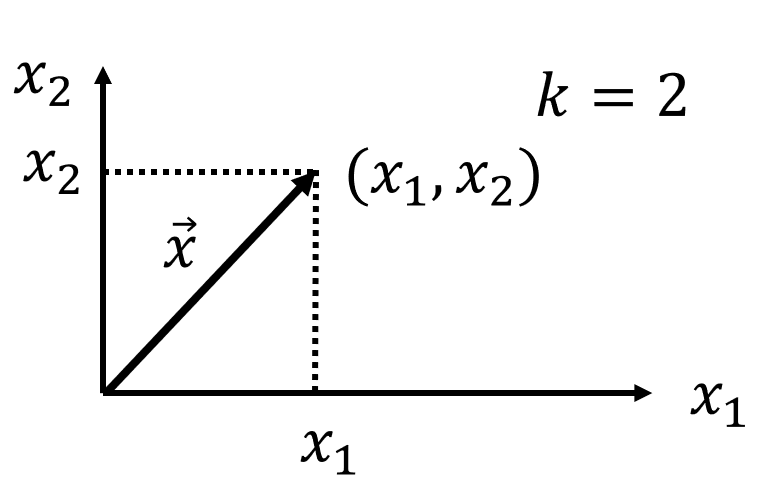
\includegraphics[width=0.9\linewidth]{image/screenshot001.png}
		\subcaption{При $k=2$}
		\label{fig:1.1.1.1}
	\end{minipage}
	\begin{minipage}{0.45\linewidth}
		\centering
		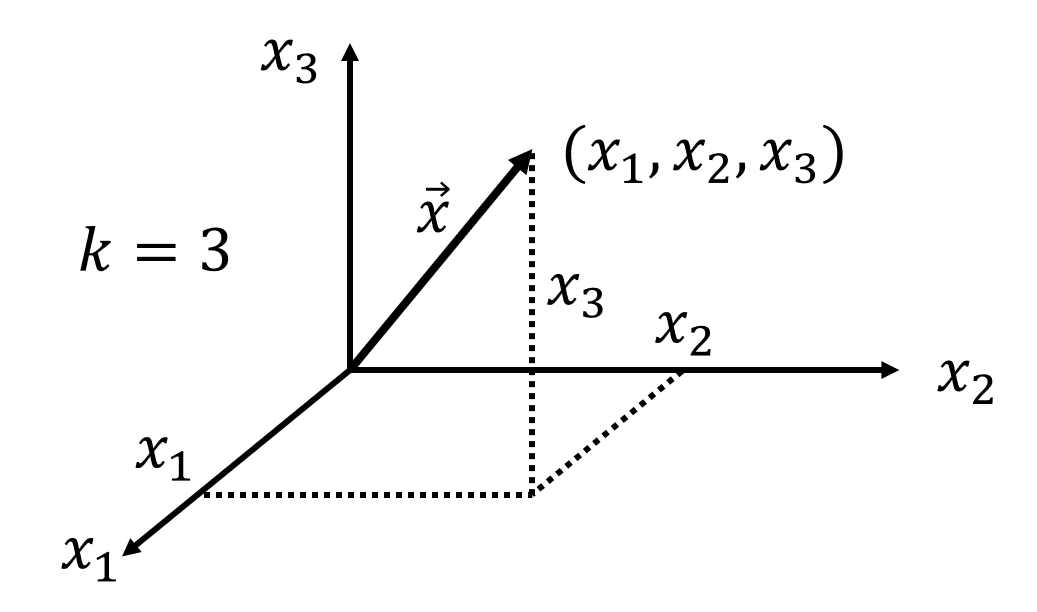
\includegraphics[width=0.9\linewidth]{image/screenshot006.png}
		\subcaption{При $k=3$}
		\label{fig:1.1.1.2}
	\end{minipage}
	\caption{Примеры $\mathbb{R}^k$ пространств}
	\label{fig:1.1.1}
\end{figure}

Аналогично, если $k=3$, то упорядоченный набор $(x_1, x_2, x_3)$ определяет точку или вектор в пространстве (\Cref{fig:1.1.1.2}).

Таким образом, элементами множества $\mathbb{R}^k$ являются \uline{векторы}. Над векторами вводятся следующие операции:
\begin{enumerate}
	\item \textbf{Сложение векторов}\\
	Если $\vec{x} = (x_1, x_2, ..., x_k) \in \mathbb{R}^k$ и $\vec{y} = (y_1, y_2, ..., y_k) \in \mathbb{R}^k$, то суммой векторов $(\vec{x} + \vec{y})$, будет являться сумма соответствующих координат:
	\begin{align} \label{1.1.1}
		(\vec{x} + \vec{y}) = (x_1 + y_1, x_2 + y_2, ..., x_k + y_k)
	\end{align}

	\item \textbf{Умножение вектора на скаляр}\\
	Если $\vec{x} = (x_1, x_2, ..., x_k)$ и $\alpha \in \mathbb R$ - действительное число, то $\alpha \vec{x} \in \mathbb{R}^k$ -- это вектор с координатами:
	\begin{align} \label{eq:1.1.2}
		(\alpha\vec{x}) = (\alpha \cdot x_1, \alpha \cdot x_2, ..., \alpha \cdot x_k)
	\end{align}

	\item \textbf{Скалярное произведение векторов}\\
	Если $\vec{x} = (x_1, x_2, ..., x_k) \in \mathbb{R}^k$ и $\vec{y} = (y_1, y_2, ..., y_k) \in \mathbb{R}^k$, тогда \textit{скалярным произведением векторов} называться скалярная величина, равная сумме произведений одноименных координат:
	\begin{align} \label{eq:1.1.3}
		(\vec{x} + \vec{y}) = x_1 y_1 + x_2 y_2 + ... + x_k y_k = \sum_{i = 1}^{k} x_i y_i
	\end{align}

	\item \textbf{Норма или длина вектора}\\
	Длина вектора $\vec{x} = (x_1, x_2, ..., x_k)$ вычисляется по формуле:
	\begin{align} \label{eq:1.1.4}
		||\vec{x}|| = \sqrt{x_1^2 + x_2^2 + ... + x_k^2} = \sqrt{\sum_{i=1}^{k} x_i^2}
	\end{align}

	\item \textbf{Расстояние между двумя точками или векторами}\\
	Если $\vec{x} = (x_1, x_2, ..., x_k) \in \mathbb{R}^k$ и $\vec{y} = (y_1, y_2, ..., y_k) \in \mathbb{R}^k$, то расстояние между точками $\rho(\vec{x}, \vec{y})$ определяется длиной вектора $(\vec{x} - \vec{y})$:
	\begin{multline} \label{eq:1.1.5}
		\rho(\vec{x}, \vec{y}) = ||\vec{x} - \vec{y}|| = \sqrt{(x_1 - y_1)^2 + (x_2 - y_2)^2 + ... + (x_k - y_k)^2} = \\ = \sqrt{\sum_{i=1}^{k} (x_i - y_i)^2}
	\end{multline}
\end{enumerate}

Если в множестве $\mathbb{R}^k$ введены рассмотренные выше операции с векторами, то оно называется \textbf{k-мерным Евклидовым пространством}.
	\subsection{Понятие функции многих переменных} \label{sec:1.2}

Начнем с определения функции одной переменной.

Если каждому числу $x$ из множества $\mathbb{E}$, которое является подмножеством действительных чисел $\mathbb{R}$, соответствует число $y$ из множества $Y$, также являющегося подмножеством $\mathbb{R}$ в соответствии с правилом $f$, то говорят, что на множестве $\mathbb{E}$ задана функция $y = f(x)$. Множество $\mathbb{E}$ называют областью определения функции, а $Y$ — множеством её значений.\\

Функция нескольких переменных определяется аналогично, только вместо одного числа используются несколько независимых переменных.

\begin{tbox*}{Определение функции k независимых переменных}
	Если каждому вектору $\vec{x} = (x_1, x_2, ..., x_k)$ из множества $\mathbb{E} \subset \mathbb{R}^k$ соответствует число $y$ из множества $Y \subset \mathbb{R}$ по правилу $f$, то на множестве $\mathbb{E}$ задана функция нескольких переменных, которую обозначают как $y = f(\vec{x})$ или $y = f(x_1, x_2, ..., x_k)$.

	Здесь $x_1, x_2, ..., x_k$ — независимые переменные (аргументы функции), а $y$ — зависимая переменная.

	Множество $\mathbb{E} \subset \mathbb{R}^k$ называют областью определения функции, а множество $Y \subset \mathbb{R}$ — её множеством значений.
\end{tbox*}

\subsubsection{Частные случаи функций многих переменных}
Рассмотрим функции двух и трех переменных. Для функции двух переменных:

\begin{itemize}
	\item Если $k=2$, то $y = f(x_1, x_2)$, что записывается как $z = f(x, y)$;
	\item Если $k=3$, то $y = f(x_1, x_2, x_3)$, что записывается как $w = f(x, y, z)$.
\end{itemize}

Особенно важна функция двух переменных $z = f(x, y)$, где $x$ и $y$ — независимые переменные. Область определения этой функции — множество точек $(x, y)$, принадлежащих некоторому подмножеству $\mathbb{E} \subset \mathbb{R}^2$. Зависимая переменная $z$ принимает значения из множества $Z \subset \mathbb{R}$, которое откладывается по вертикальной оси в пространстве XYZ.

По определению функции, каждой паре $(x, y) \in \mathbb{E}$ ставится в соответствие единственное значение $z$ по закону $f$. Это означает, что функция двух переменных имеет графическое представление в виде поверхности в пространстве. Эта поверхность состоит из всех значений функции во всех точках области определения $\mathbb{E}$.

\noindent
\begin{minipage}{\linewidth}
	\begin{minipage}{0.6\linewidth}
		\begin{tbox*}{Параболоид вращения (\Cref{fig:1.2.1.1})}
			\[\boxed{z = x^2 + y^2}\]
			О.О. $(x, y) \in \mathbb{R}$, $z \geqslant 0$ - множество значений
		\end{tbox*}
	\end{minipage}
	\begin{minipage}{0.35\linewidth}
		\begin{figure}[H]
			\centering
			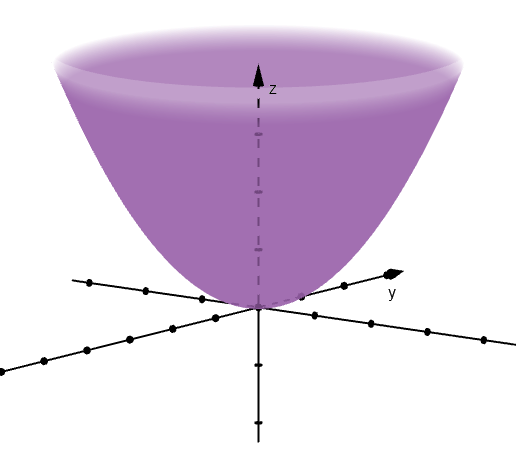
\includegraphics[width=0.9\linewidth]{image/screenshot004.png}
			\caption{Параболоид}
			\label{fig:1.2.1.1}
		\end{figure}
	\end{minipage}
\end{minipage}
\begin{minipage}{\linewidth}
	\begin{minipage}{0.6\linewidth}
		\begin{tbox*}{Коническая поверхность (\Cref{fig:1.2.1.2})}
			\[\boxed{z^2 = x^2 + y^2}\]

			-- это неявно заданная функция. Выразим из уравнения $z$, $z = \pm \sqrt{x^2 + y^2}$ - получаем две явно заданные функции:
			\begin{enumerate}
				\item $\boxed{z = \sqrt{x^2 + y^2}}$, $(x, y) \in \mathbb{R}^2$, $z \geqslant 0$
				\item $\boxed{z = -\sqrt{x^2 + y^2}}$, $(x, y) \in \mathbb{R}^2$, $z \leqslant 0$
			\end{enumerate}
		\end{tbox*}
	\end{minipage}
	\begin{minipage}{0.35\linewidth}
		\begin{figure}[H]
			\centering
			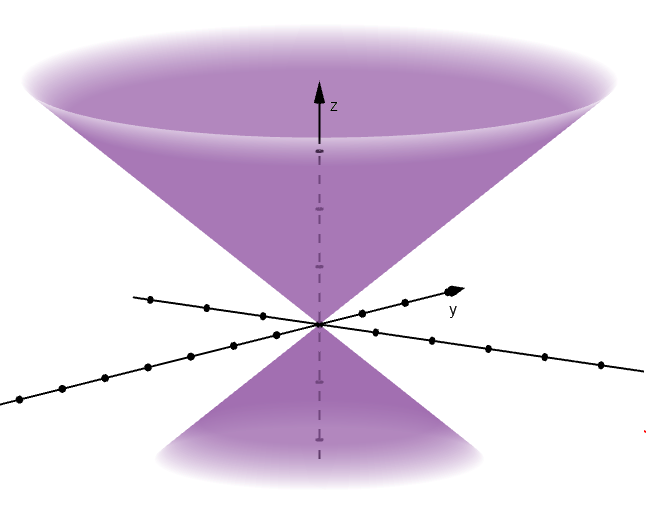
\includegraphics[width=0.9\linewidth]{image/screenshot005.png}
			\caption{Коническая поверхность}
			\label{fig:1.2.1.2}
		\end{figure}
	\end{minipage}
\end{minipage}
\begin{minipage}{\linewidth}
	\begin{minipage}{0.6\linewidth}
		\begin{tbox*}{Сфера с цетром в начале (\Cref{fig:1.2.1.3})}
			\[\boxed{x^2 + y^2 + z^2 = R^2}\]

			Функция $z = \sqrt{R^2 - x^2 - y^2}$ задает верхнюю половину сферы. Здесь область определения $R^2 -x^2 - y^2 \geqslant 0 \Rightarrow x^2 + y^2 \leqslant R^2$ - круг радиуса $R$, а множество значений $0 \leqslant z \leqslant R$.\\

			Функция $z = -\sqrt{R^2 - x^2 - y^2}$ задает нижнюю половину сферы, область определения $x^2 + y^2 \leqslant R^2$, а множество значений $-R \leqslant z \leqslant 0$.\\

			\textbf{Замечание: } Функции, большего числа переменных, не имеют геометрического изображения.
		\end{tbox*}
	\end{minipage}
	\begin{minipage}{0.35\linewidth}
		\begin{figure}[H]
			\centering
			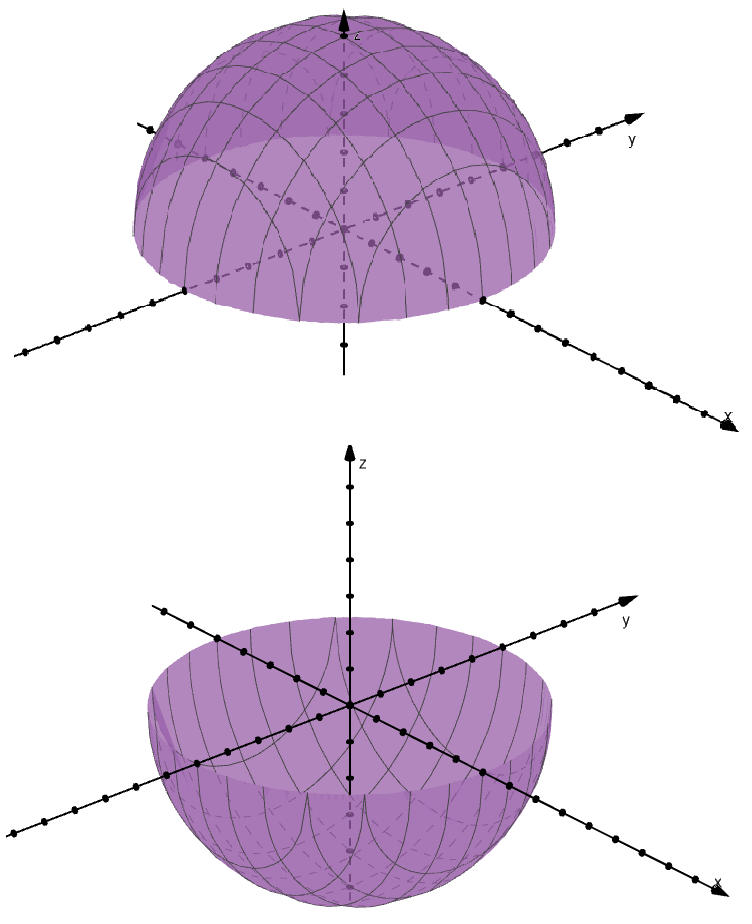
\includegraphics[width=0.9\linewidth]{image/screenshot007.png}
			\caption{Сфера с цетром в начале}
			\label{fig:1.2.1.3}
		\end{figure}
	\end{minipage}
\end{minipage}

	\subsection{Понятие предела функции многих переменных}
\begin{tbox}{Предел функции одной переменной}
	Вспомним определение предела для функции одной действительной переменной. Пусть \( y = f(x) \), где \( x \in \mathbb{E} \subset \mathbb{R} \). Точка \( x = a \) является предельной точкой множества \( \mathbb{E} \); она может как принадлежать \( \mathbb{E} \), так и не принадлежать ему (\( a \in \mathbb{E} \) или \( a \notin \mathbb{E} \)).

	\begin{multline} \label{eq:1.3.1}
		\lim_{x \to a} f(x) = A \Leftrightarrow
		(\forall \varepsilon > 0) \, (\exists \delta = \delta(\varepsilon) > 0) \,
		(\forall x \in \mathbb{E}, \, 0 < |x - a| < \delta) : \\
		|f(x) - A| < \varepsilon
	\end{multline}

	В определении предела неравенство \( 0 < |x - a| < \delta \) означает, что \( x \in (a - \delta, a + \delta) \) и \( x \neq a \). Геометрический смысл модуля \( |x - a| = \rho(x, a) \) — это расстояние между точками \( x \) и \( a \) на действительной оси, причём \( 0 < \rho(x, a) < \delta \).
\end{tbox}

\begin{tbox}{Предел функции многих переменных}
	Обобщим определение предела на случай функции многих переменных. Пусть \( y = f(\vec{x}) = f(x_1, x_2, \dots, x_k) \) определена на множестве \( \mathbb{E} \subset \mathbb{R}^k \). Точка \( \vec{a} = (a_1, a_2, \dots, a_k) \) является предельной для \( \mathbb{E} \) и может как принадлежать \( \mathbb{E} \), так и не принадлежать ему (\( \vec{a} \in \mathbb{E} \) или \( \vec{a} \notin \mathbb{E} \)).

	Расстояние между точками в \( \mathbb{R}^k \) было введено в \cref{sec:1.1}:
	\begin{align}
		\rho(\vec{x}, \vec{a}) = \|\vec{x} - \vec{a}\| =
		\sqrt{(x_1 - a_1)^2 + (x_2 - a_2)^2 + \dots + (x_k - a_k)^2}.
	\end{align}

	Предел функции многих переменных обозначается следующим образом:
	\begin{align}
		\lim_{\vec{x} \to \vec{a}} f(\vec{x}) = A \quad \text{или} \quad
		\lim_{\substack{x_1 \to a_1 \\ x_2 \to a_2 \\ \vdots \\ x_k \to a_k}}
		f(x_1, x_2, \dots, x_k) = A.
	\end{align}

	На языке «\(\varepsilon\)-\(\delta\)» определение аналогично \cref{eq:1.3.1}, но вместо чисел \( x \) и \( a \) используются векторы \( \vec{x} \) и \( \vec{a} \), а модуль \( |x - a| \) заменяется на норму \( \|\vec{x} - \vec{a}\| \):
	\begin{align}
		(\forall \varepsilon > 0) \, (\exists \delta = \delta(\varepsilon) > 0) \,
		(\forall \vec{x} \in \mathbb{E}, \, 0 < \|\vec{x} - \vec{a}\| < \delta) :
		|f(\vec{x}) - A| < \varepsilon
		\label{eq:2}
	\end{align}
\end{tbox}

\begin{tbox*}{Замечание о пределах}
	\textbf{Замечание.} Поскольку определение предела \eqref{eq:2} для функции многих переменных совпадает с определением для функции одной переменной, все теоремы о пределах, доказанные для случая одной переменной, переносятся на случай многих переменных.
\end{tbox*}

\begin{tbox}{Двойной предел}
	Рассмотрим предел функции двух переменных \( z = f(x, y) \), называемый двойным пределом. Пусть точка \( M(x, y) \in \mathbb{E} \subset \mathbb{R}^2 \) принадлежит области определения функции, а точка \( M_0(a, b) \) является предельной для \( \mathbb{E} \) (\( M_0 \in \mathbb{E} \) или \( M_0 \notin \mathbb{E} \)). Тогда:
	\begin{align}
		A = \lim_{M \to M_0} f(x, y) =
		\lim_{\substack{x \to a \\ y \to b}} f(x, y).
	\end{align}

	Расстояние между точками \( M \) и \( M_0 \) вычисляется по формуле:
	\[
	\rho(M, M_0) = \sqrt{(x - a)^2 + (y - b)^2} < \delta.
	\]

	На языке «\(\varepsilon\)-\(\delta\)» двойной предел записывается так:
	\begin{align}
		(\forall \varepsilon > 0) \, (\exists \delta = \delta(\varepsilon) > 0) \,
		(\forall (x, y) \in \mathbb{E}, \, 0 < \sqrt{(x - a)^2 + (y - b)^2} < \delta) : \\
		|f(x, y) - A| < \varepsilon
		\label{eq:3}
	\end{align}
\end{tbox}
\begin{figure}[t]
	\centering
	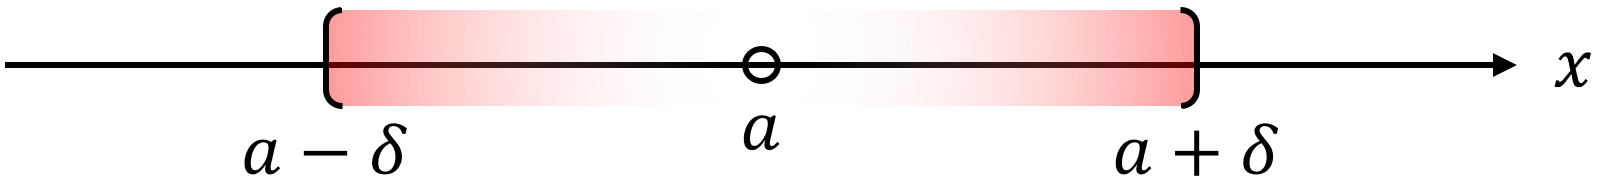
\includegraphics[width=0.7\linewidth]{image/screenshot008}
	\caption{Интервал $(a - \delta, a + \delta)$ с выколотой точкой}
	\label{fig:1.3.1}
\end{figure}
\begin{tbox}{Геометрический смысл двойного предела}
	Рассмотрим геометрический смысл неравенства:
	\begin{gather}
		0 < \sqrt{(x - a)^2 + (y - b)^2} < \delta = \delta(\varepsilon), \\
		0 < (x - a)^2 + (y - b)^2 < \delta^2(\varepsilon).
	\end{gather}

	Это задаёт круг радиуса \( \delta(\varepsilon) \) с выколотым центром в точке \( M_0(a, b) \). Такой круг называют \(\delta\)-окрестностью точки \( M_0 \) (\Cref{fig:1.3.2.1}).

	Для сравнения: в случае функции \( y = f(x) \) \(\delta\)-окрестность точки \( a \) — это интервал \( (a - \delta, a + \delta) \) с выколотой точкой \( a \) (\Cref{fig:1.3.1}).
\end{tbox}

\begin{tbox}{Независимость предела от пути}
	Из определения двойного предела следует, что если предел существует, то он не зависит от пути, по которому точка \( M \) приближается к \( M_0 \). Число возможных направлений бесконечно, в отличие от функции одной переменной, где таких направлений всего два (слева и справа от точки \( a \)).
\end{tbox}

\begin{figure}[H]
	\centering
	\begin{minipage}{0.45\linewidth}
		\centering
		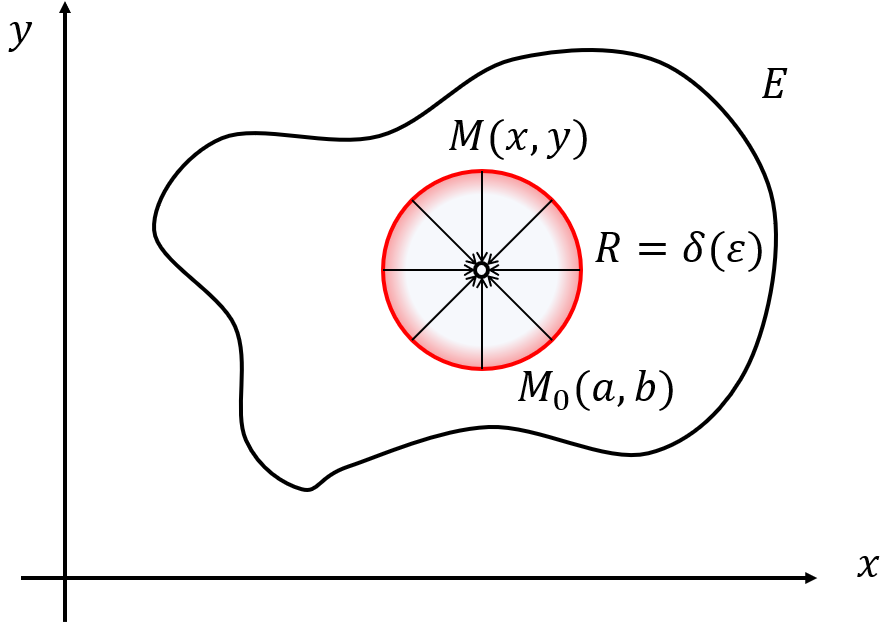
\includegraphics[width=0.9\linewidth]{image/screenshot009.png}
		\caption{ }
		\label{fig:1.3.2.1}
	\end{minipage}
	\begin{minipage}{0.45\linewidth}
		\centering
		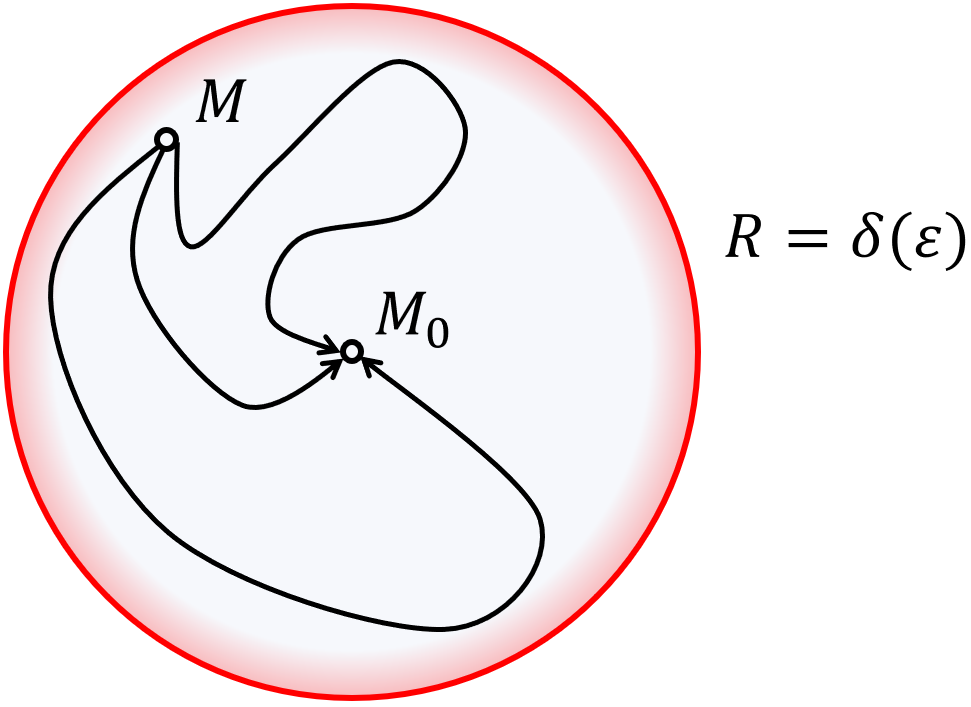
\includegraphics[width=0.9\linewidth]{image/screenshot010.png}
		\caption{ }
		\label{fig:1.3.2.2}
	\end{minipage}
\end{figure}

\subsubsection{Примеры решения двойных пределов}
\begin{enumerate}
	\item Вместо $x$ и $y$ подставляем предельные значения:
	\begin{align*}
		\lim_{\tiny{\begin{array}[b]{c} x \to 1\\y \to 2 \end{array}}} \frac{x \cdot y}{x^2 + y^2} =
		\frac{1 \cdot 2}{1^2 + 2^2} =
		\frac{2}{5}
	\end{align*}

	\item По теореме и произведении бесконечно малых на ограниченную:
	\begin{align*}
		\lim_{\tiny{\begin{array}[b]{c} x \to 0\\y \to 0 \end{array}}} (x + y \cdot \sin \frac{1}{x}) =
		\lim_{x \to 0} x + \lim_{\tiny{\begin{array}[b]{c} x \to 0\\y \to 0 \end{array}}} y \cdot \sin \frac{1}{x} =
		0
	\end{align*}

	\item Используя первый замечательный предел:
	\begin{multline*}
		\lim_{\tiny{\begin{array}[b]{c} x \to \infty \\y \to 2 \end{array}}} \left(x \cdot \sin \frac{1}{xy}\right) \, [\infty \cdot 0] =
		\lim_{\tiny{\begin{array}[b]{c} x \to \infty \\y \to 2 \end{array}}} \left(\frac{\sin \frac{1}{xy}}{\frac{1}{x}}\right) \left[\frac{0}{0}\right] =\\=
		\lim_{\tiny{\begin{array}[b]{c} x \to \infty \\y \to 2 \end{array}}} \left(\frac{\sin \frac{1}{xy}}{\frac{1}{xy} \cdot y}\right) =
		\lim_{y \to 2} \frac{1}{y} = \frac{1}{2}
	\end{multline*}

	\item Покажем что предел не существует. Для этого выберем окрестность предельной точки $M_0(0,0)$ и предположим, что точка $M(x, y) \to M_0(0, 0)$ по различным путям (выше уже было сказано, что число таких направлений бесконечно). Для простоты выберем две прямые: $y = x$ и $y = -x$
	\begin{align*}
		\lim_{\tiny{\begin{array}{c} x \to 0 \\[-3pt] y \to 0 \end{array}}} \frac{xy}{x^2 + y^2}
		= \left| \begin{array}{l} y = x \\[-3pt] x \to 0 \\[-3pt] y \to 0 \end{array} \right| = \lim_{x \to 0} \frac{x^2}{x^2 + x^2} = \lim_{x \to 0} \frac{x^2}{2x^2} = \frac{1}{2}
	\end{align*}
	\begin{align*}
		\lim_{\tiny{\begin{array}{c} x \to 0 \\[-3pt] y \to 0 \end{array}}} \frac{xy}{x^2 + y^2}
		= \left| \begin{array}{l} y = -x \\[-3pt] x \to 0 \\[-3pt] y \to 0 \end{array} \right| = \lim_{x \to 0} \frac{x \cdot (-x)}{x^2 + (-x)^2} = \lim_{x \to 0} \frac{x^2}{2x^2} = -\frac{1}{2}
	\end{align*}
	Таким образом, рассмотрели 2 частных предела, они не равны между собой, следовательно двойной предел не существует.
\end{enumerate}
	\subsection{Понятие непрерывности функции многих переменных}

\begin{tbox}{Непрерывность функции одной переменной}
	Вспомним определение непрерывной функции одного действительного переменного. Функция \(y = f(x)\), где \(x \in E \subset \mathbb{R}\), называется непрерывной в точке \(x_0 \in E\), если $\lim_{x \to x_0} f(x) = f(x_0)$, то есть предел \(f(x)\) при \(x \to x_0\) равен значению функции в точке \(x_0\). \\

	В этом случае предельная точка \(x_0 \in E\), поэтому на языке \(\varepsilon - \delta\)-определение принимает вид:
	\begin{align} \label{eq:1.4.1}
		(\forall \varepsilon > 0)(\exists \delta = \delta(\varepsilon) > 0)(\forall x \in E \subset \mathbb{R}, \, |x - x_0| < \delta): \, |f(x) - f(x_0)| < \varepsilon
	\end{align}
\end{tbox}

\begin{tbox}{Приращение функции одной переменной}
	Если в определении (\ref{eq:1.4.1}) \((x - x_0 = \Delta x)\) приращение аргумента, $f(x) - f(x_0) = \Delta f(x_0)$ -- приращение функции, то определение (\ref{eq:1.4.1}) можно записать в виде:
	\begin{align} \label{eq:1.4.2}
		(\forall \varepsilon > 0)(\exists \delta = \delta(\varepsilon) > 0)(\forall x \in E \subset \mathbb{R}, \, |\Delta x| < \delta): \, |\Delta f(x_0)| < \varepsilon
	\end{align}

	Поэтому из непрерывной функции малым приращением аргумента соответствуют малые приращения функции.
\end{tbox}

\begin{tbox}{Непрерывность функции многих переменных}
	Обобщим определения непрерывности функции одной переменной на случай функции многих переменных. Пусть на множестве \(E \subset \mathbb{R}^k\) задана функция \(y=f(\vec{x})\), где $\vec{x} = (x_1, x_2, ..., x_k) \in E \subset \mathbb{R}^k$ и пусть $\vec{x}_0 = (x_\text{$0_1$}, x_\text{$0_2$}, ..., x_\text{$0_k$}) \in E \subset \mathbb{R}^k$ - предельная точка множества $E$.\\

	Функция $y = f(\vec{x})$ называется непрерывной в точке $\vec{x}_0$, если:
	\begin{align} \label{eq:1.4.3}
		\lim_{\vec{x} \to \vec{x}_0} f(\vec{x}) = f(\vec{x}_0) \qquad \lim_{\tiny{\begin{array}[b]{c}x_1 \to a_1\\x_2 \to a_1\\ \cdots \\ x_k \to a_k\end{array}}} f(x_1, x_2, ..., x_k) = f(x_\text{$0_1$}, x_\text{$0_2$}, ..., x_\text{$0_k$})
	\end{align}
\end{tbox}

\begin{tbox}{Непрерывность на языке $\varepsilon - \delta$}
	На языке <<$\varepsilon - \delta$>> это определение получается из определения (\ref{eq:1.4.1}) при замене $x \to \vec{x}$, $x_0 \to \vec{x}_0$ и $|x - x_0| \to ||\vec{x} - \vec{x}_0||$.
	\begin{align} \label{eq:1.4.4}
		(\forall \varepsilon > 0)(\exists \delta = \delta(\varepsilon) > 0)(\forall \vec{x} \in E \subset \mathbb{R}^k, \, ||\vec{x} - \vec{x}_0|| < \delta): \, |f(\vec{x}) - f(\vec{x}_0)| < \varepsilon
	\end{align}
\end{tbox}

\begin{tbox}{Приращение аргументов и функции}
	В определении (\ref{eq:1.4.4}) обозначим:
	\begin{align}
		\Delta \vec{x} = \vec{x} - \vec{x}_0 = (x_1 - x_\text{$0_1$}, x_2 - x_\text{$0_2$}, ..., x_k - x_\text{$0_k$}) = (\Delta x_1, \Delta x_2, ..., \Delta x_k)
	\end{align}
	--- вектор приращения аргументов.
	\begin{align} \label{eq:1.4.5}
		\Delta f(\vec{x}) = f(\vec{x}) - f(\vec{x}_0)
	\end{align}
	--- приращение функции, аналогичное (\ref{eq:1.4.2}), только здесь $\Delta x$ заменяем на вектор $\Delta \vec{x}$, и соответственно $|\Delta x|$ заменяем на $||\Delta \vec{x}||$.
	\begin{align} \label{eq:1.4.6}
		(\forall \varepsilon > 0)(\exists \delta = \delta(\varepsilon) > 0)(\forall \vec{x} \in E \subset \mathbb{R}^k, \, ||\Delta \vec{x}|| < \delta): \, |\Delta f(\vec{x}_0)| < \varepsilon
	\end{align}
	--- здесь \(||\Delta \vec{x}|| = \sqrt{(\Delta x_1)^2 + (\Delta x_2)^2 + ... + (\Delta x_k)^2}\).
\end{tbox}

\begin{tbox}{Полное приращение функции}
	Если дать приращение переменной $\vec{x}$ в точке $\vec{x}_0$ по все независимым переменным одновременной т.е. $\vec{x} - \vec{x}_0 = \Delta \vec{x} \Rightarrow \vec{x} = \vec{x}_0 + \Delta \vec{x} = (x_1 + x_\text{$0_1$}, x_2 + x_\text{$0_2$}, ..., x_k + x_\text{$0_k$})$, то приращение, которое получит функция $f(\vec{x})$ в точке $\vec{x}_0$ называется полным приращением функции (\ref{eq:1.4.7}).
	\begin{multline} \label{eq:1.4.7}
		\Delta f(\vec{x}_0) = f(\vec{x}) - f(\vec{x}_0) = f(\vec{x}_0 + \Delta \vec{x}) =\\= f(x_1 + x_\text{$0_1$}, x_2 + x_\text{$0_2$}, ..., x_k + x_\text{$0_k$}) - f(x_\text{$0_1$}, x_\text{$0_2$}, ..., x_\text{$0_k$})
	\end{multline}
\end{tbox}

\begin{tbox}{Непрерывность по совокупности переменных}
	Тогда определение непрерывности (\ref{eq:1.4.6}) словами можно сформулировать так:

	Функция $y = f(\vec{x})$ непрерывна в точке $\vec{x}_0$ по совокупности переменные (т.е. по всем  переменным $x_1, x_2, ..., x_k$ одновременно), если малым приращениям всех независимых переменных соответствует малое полное приращение функции.
\end{tbox}

\begin{tbox}{Частное приращение функции}
	Для функции многих переменных приращение аргумента можно давать также только по отдельности переменной. Обозначим ее $x_i$, где $i=1,2,..., \vec{k}$, что означает либо по $x_1$, либо по $x_2$, ..., либо по $x_k$. Вектор приращений аргументов в этом случае принимает вид:
	\[\Delta \vec{x} = (0, ..., 0, \Delta x_i, 0, ..., 0)\]
	\[\vec{x} = \vec{x}_0 + \Delta \vec{x} = (x_\text{$0_1$}, ..., x_\text{$0_{i - 1}$}, x_\text{$0_i$} + \Delta x_i, x_\text{$0_{i + 1}$}, ..., x_\text{$0_k$})\]

	Тогда приращение, которое получит функция в этом случае, называется \uline{частным приращением функции} в точке $\vec{x}_0$ по переменной $x_i$ и обозначается $\Delta_i f(\vec{x}_0)$:
	\begin{multline} \label{eq:1.4.8}
		\Delta_i f(\vec{x}_0) = f(\vec{x}_0 + \Delta \vec{x}) - f(\vec{x}_0) = f(x_\text{$0_1$}, \cdots, x_\text{$0_{i - 1}$}, x_\text{$0_i$} + \Delta x_i, x_\text{$0_{i + 1}$}, \cdots, x_\text{$0_k$}) - \\
		-f(x_\text{$0_1$}, \cdots, x_\text{$0_{i-1}$}, x_\text{$0_i$}, x_\text{$0_{i+1}$}, \cdots, x_\text{$0_k$})
	\end{multline}
\end{tbox}

\begin{tbox}{Непрерывность по отдельной переменной}
	Функция $y = f(\vec{x})$ называется \uline{непрерывной в точке $\vec{x}_0$ по отдельной переменной $x_i$}, если:
	\begin{multline} \label{eq:1.4.9}
		\lim_{x_i \to x_\text{$0_i$}} f(x_\text{$0_1$}, ..., x_\text{$0_{i-1}$}, x_\text{$0_i$}, x_\text{$0_{i+1}$}, ..., x_\text{$0_k$}) =\\= f(x_\text{$0_1$}, ..., x_\text{$0_{i-1}$}, x_\text{$0_i$}, x_\text{$0_{i+1}$}, ..., x_\text{$0_k$}),
	\end{multline}
	здесь $i = \bar{1, k}$, т.е. функция может быть непрерывной, либо по переменной $x_1$, либо $x_2$, ..., либо по $x_k$. В этом случае:
	\begin{align}
		||\Delta \vec{x}|| = \sqrt{0 + ... + 0 + (\Delta x_i)^2 + ... + 0} = \sqrt{(\Delta x_i)^2} = |\Delta x_i|
		\label{eq:1.4.10}
	\end{align}
	Тогда определение (\ref{eq:1.4.6}) принимает вид и значит:
	\begin{align}
		(\forall \varepsilon > 0)(\exists \delta = \delta(\varepsilon) > 0)(\forall \vec{x} \in E \subset \mathbb{R}^k, \, |\Delta x_i| < \delta): \, |\Delta_i f(\vec{x}_0)| < \varepsilon
		\label{eq:1.4.11}
	\end{align}

	Функция $y=f(\vec{x})$ называется \uline{непрерывной в точке $\vec{x}_0$ по переменной $x_i$}, если \uline{малым приращением этой переменной $\Delta x_i$}, соответствует \uline{малое частное приращение функции $\Delta_i f(\vec{x}_0)$}.
\end{tbox}

\begin{tbox}{Теорема и замечание}
	\textbf{Теорема (без доказательства)} \\
	Если функция $y=f(\vec{x})$ непрерывна в точке $\vec{x}_0$ по совокупности переменных, то она будет непрерывна и по каждой переменной в отдельности. Обратно утверждение не всегда верно.

	\textbf{Замечание} \\
	Если функция $y = f(\vec{x})$ непрерывна по совокупности переменных, то для нее будет выполняться все теоремы о непрерывности, доказанные для функции одной переменной.
\end{tbox}

	\newpage
	\section{Дифференцирование функций многих переменных}
	\subsection{Определение частных производных и их геометрический смысл} \label{sec:2.1}

\begin{tbox}{Функция одной переменной}
	Рассмотрим функцию \( y = f(x) \), где \( x \in E \subset \mathbb{R} \) и \( y \in E \).
	Запишем определение производной в точке \( x_0 \). Для этого зададим приращение аргумента \( \Delta x = x - x_0 \) (или \( x = x_0 + \Delta x \)) и вычислим приращение функции:
	\[
	\Delta f(x_0) = f(x_0 + \Delta x) - f(x_0).
	\]

	Производной функции в точке называется предел отношения приращения функции к приращению аргумента при \( \Delta x \to 0 \):
	\begin{align}
		\lim_{\Delta x \to 0} \frac{\Delta f(x_0)}{\Delta x} = f'(x_0) = \frac{dy}{dx}\bigg|_{x = x_0} = \frac{df(x_0)}{dx}.
		\label{eq:15}
	\end{align}
\end{tbox}

\begin{tbox}{Функция многих переменных}
	Теперь обобщим определение (\ref{eq:15}) на случай функции многих переменных \( y = f(\vec{x}) = f(x_1, x_2, \dots, x_k) \). Поскольку дифференцирование проводится по одной переменной, зададим приращение в точке \( \vec{x}_0 \) только по переменной \( x_i \). Вектор приращений имеет вид:
	\[
	\Delta \vec{x} = (0, \dots, 0, \Delta x_i, 0, \dots, 0),
	\]

	тогда:
	\[
	\vec{x} = \vec{x}_0 + \Delta \vec{x} = \left(x_0^{(1)}, \dots, x_0^{(i-1)}, x_0^{(i)} + \Delta x_i, x_0^{(i+1)}, \dots, x_0^{(k)}\right).
	\]

	Соответствующее частное приращение функции:
	\begin{align}
		\Delta_i f(\vec{x}_0) = f\left(x_{0_1}, \dots, x_{0_{i-1}}, x_{0_i} + \Delta x_i, x_{0_{i+1}}, \dots, x_{0_k}\right) - f\left(x_{0_1}, \dots, x_{0_k}\right).
		\label{eq:16}
	\end{align}
\end{tbox}

\begin{tbox}{Частная производная}
	По аналогии с \cref{eq:15} определим частную производную как предел:
	\begin{align}
		\exists \lim_{\Delta x_i \to 0} \frac{\Delta_i f(\vec{x}_0)}{\Delta x_i}.
		\label{eq:17}
	\end{align}

	Если этот предел существует, то он называется частной производной функции \( y = f(\vec{x}) \) в точке \( \vec{x}_0 \) по переменной \( x_i \) и обозначается:
	\begin{align}
		f_{x_i}^{\prime}(\vec{x}_0) = \frac{\partial f(\vec{x}_0)}{\partial x_i}.
		\label{eq:18}
	\end{align}
	\textbf{Замечание}: Запись \( \frac{df(\vec{x}_0)}{dx_i} \) не используется для частных производных.
\end{tbox}

\begin{tbox}{Частные производные первого порядка}
	Поскольку производная вычисляется по одной из \( k \) независимых переменных, функция \( y = f(x_1, x_2, \dots, x_k) \) имеет \( k \) частных производных первого порядка:
	\begin{align}
		\frac{\partial f}{\partial x_1}, \frac{\partial f}{\partial x_2}, \dots, \frac{\partial f}{\partial x_k}.
		\label{eq:19}
	\end{align}
\end{tbox}

\begin{tbox}{Функция двух переменных}
	Рассмотрим частный случай \( z = f(x, y) \). В точке \( M_0(x_0, y_0) \) зададим приращение \( \Delta x \) по переменной \( x \). Частное приращение:
	\begin{align}
		\Delta_x z(M_0) = f(x_0 + \Delta x, y_0) - f(x_0, y_0).
		\label{eq:20}
	\end{align}

	Частная производная по \( x \):
	\begin{align}
		\frac{\partial z(M_0)}{\partial x} = \lim_{\Delta x \to 0} \frac{\Delta_x z(M_0)}{\Delta x}.
		\label{eq:21}
	\end{align}

	Аналогично для приращения \( \Delta y \) по \( y \):
	\begin{align}
		\frac{\partial z(M_0)}{\partial y} = \lim_{\Delta y \to 0} \frac{f(x_0, y_0 + \Delta y) - f(x_0, y_0)}{\Delta y}.
		\label{eq:22}
	\end{align}
\end{tbox}

\begin{tbox*}{Правила вычисления}
	При вычислении \( \frac{\partial z}{\partial x} \) переменная \( y \) считается константой, и наоборот. Используются стандартные правила дифференцирования:
	\begin{itemize}
		\item Производная константы равна нулю.
		\item Константа выносится за знак производной.
	\end{itemize}
\end{tbox*}

\begin{tbox}{Геометрический смысл}
	Функция \( z = f(x, y) \) задаёт поверхность в \( \mathbb{R}^3 \). Точке \( M_0(x_0, y_0) \) соответствует точка \( N(x_0, y_0, z_0) \) на поверхности.\\

	\textbf{Производная по x (\Cref{fig:2.1.1.1})}. При \( y = y_0 \) получаем сечение поверхности плоскостью, параллельной \( XOZ \). Частная производная \( \frac{\partial z}{\partial x} \) равна тангенсу угла \( \alpha \) наклона касательной к этому сечению:
	\[
	\tg \alpha = \frac{\partial z(M_0)}{\partial x}.
	\]

	\textbf{Производная по y (\Cref{fig:2.1.1.2})}. Аналогично, при \( x = x_0 \):
	\[
	\tg \beta = \frac{\partial z(M_0)}{\partial y}.
	\]
\end{tbox}

\begin{figure}[H]
	\centering
	\begin{minipage}{0.45\linewidth}
		\centering
		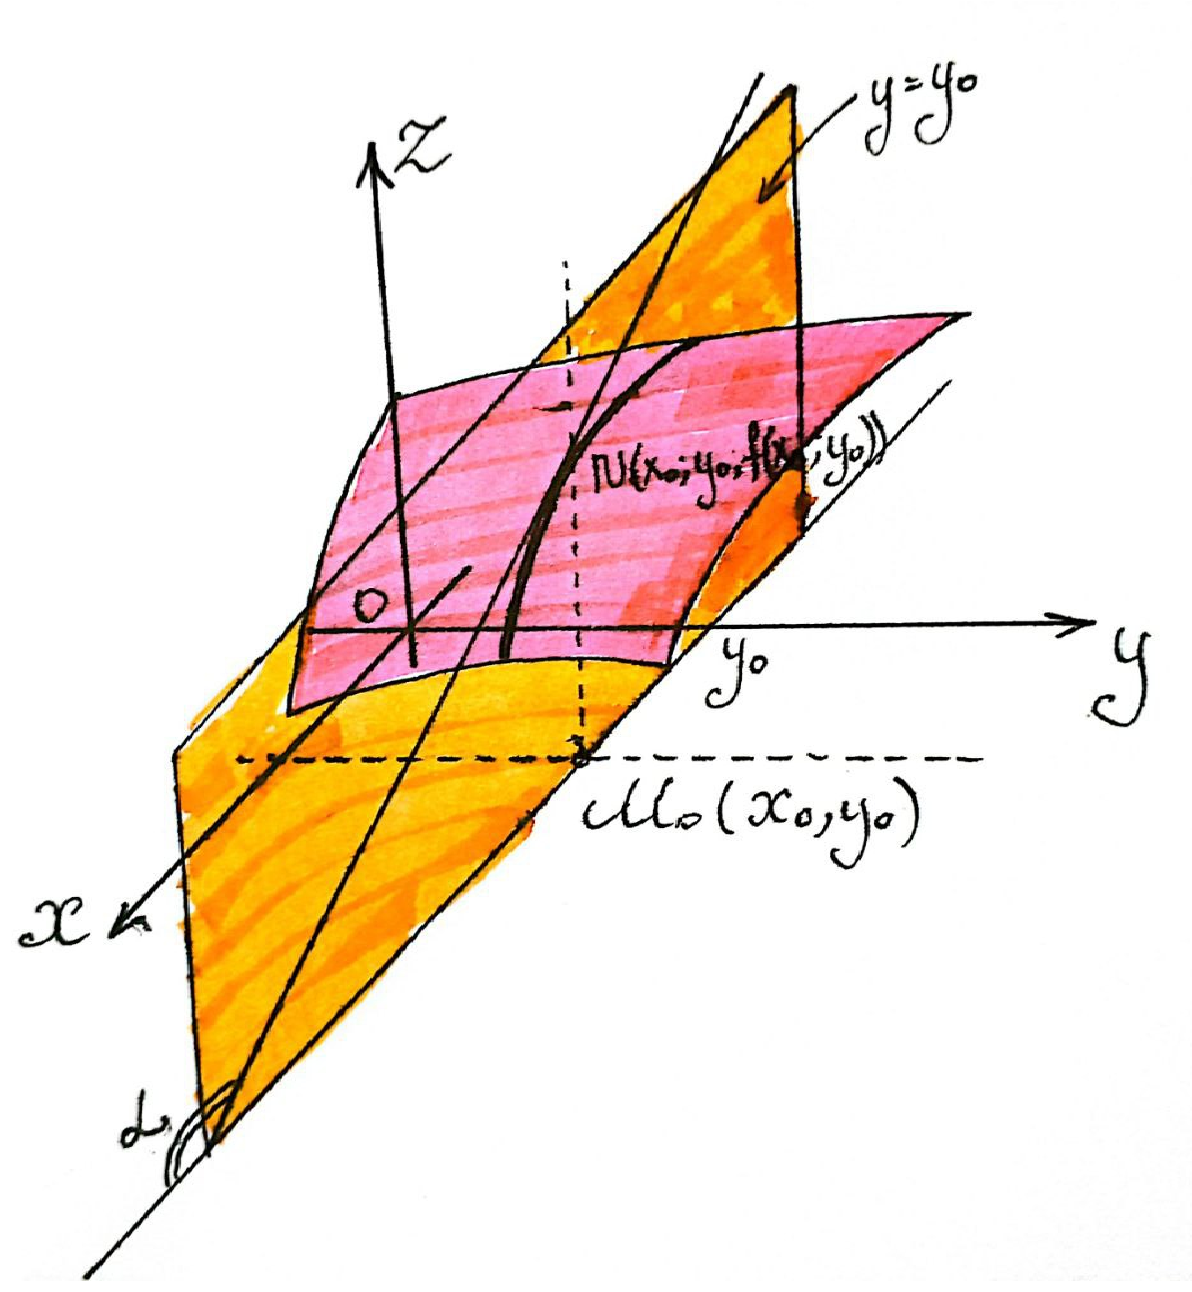
\includegraphics[width=0.9\linewidth]{screenshot011}
		\caption{Геометрический смысл \( \frac{\partial z}{\partial x} \).}
		\label{fig:2.1.1.1}
	\end{minipage}
	\begin{minipage}{0.45\linewidth}
		\centering
		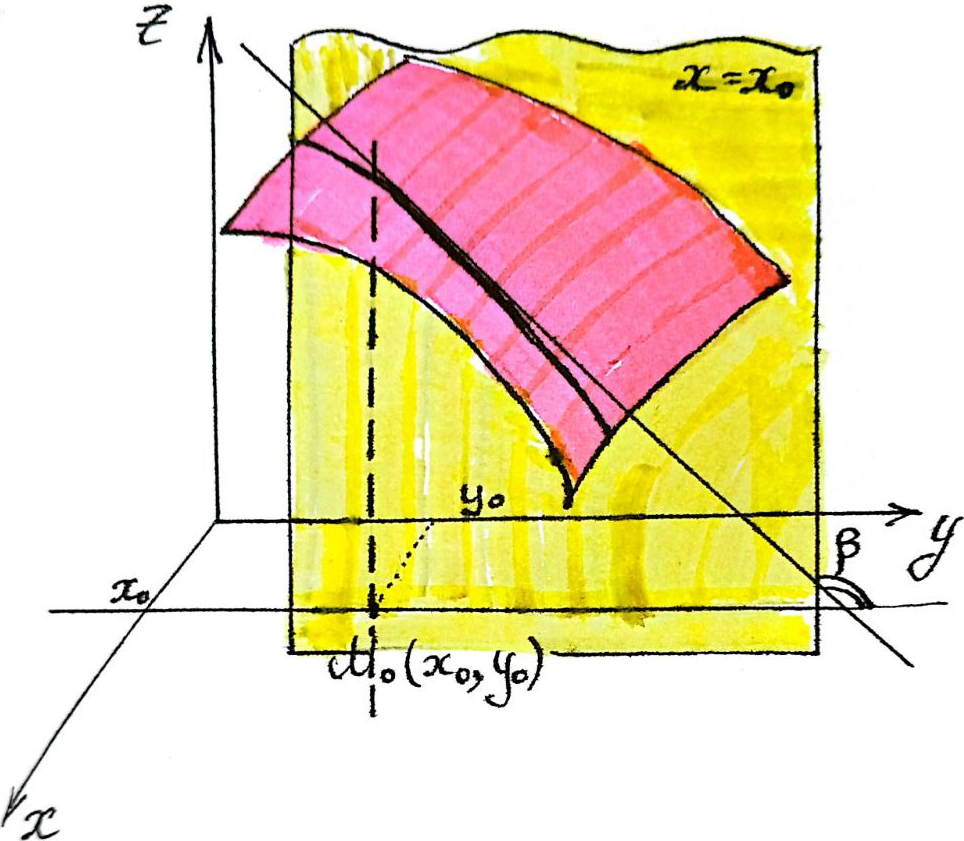
\includegraphics[width=0.9\linewidth]{screenshot012}
		\caption{Геометрический смысл \( \frac{\partial z}{\partial y} \).}
		\label{fig:2.1.1.2}
	\end{minipage}
\end{figure}
	\subsection{Дифференцируемые функции} \label{sec:2.2}

\begin{tbox}{Определение дифференцируемой функции $y = f(x)$ в точке $x_0$}
	Функция $y = f(x)$ называется \textbf{дифференцируемой в точке} \( x_0 \), если её приращение в этой точке представимо в виде:
	\begin{align} \label{eq:2.2.1}
		\Delta f(x_0) = f(x_0 + \Delta x) - f(x_0) = A \cdot \Delta x + \alpha(\Delta x) \to 0
	\end{align}
	где $A = const$, $\alpha(\Delta x)$ - бесконечно малая при \(\Delta x \to 0\), т.е. $\alpha(\Delta x) \cdot \Delta x$ -- величина бесконечно малая, более высокого порядка малости, чем $\Delta x$.
\end{tbox}

\begin{tbox}{Необходимое и достаточное условие дифференцируемости функции одной переменной}
	Существование конечной производной в точке $x_0$.\\

	Было доказано, что $A = f^{\prime}(x_0)$ и определение дифференцируемой функции можно представить следующим образом:
	\begin{align} \label{eq:2.2.2}
		\Delta f(x_0) = f^{\prime}(x_0) \cdot \Delta x + \alpha(\Delta x) \cdot \Delta x \qquad \alpha (\Delta x) \cdot \Delta x = O(\Delta x)
	\end{align}
\end{tbox}

\begin{tbox}{Определение функции многих переменных $y = f(\vec{x})$}
	Функция $\boxed{y = f(\vec{x})} = f(x_1, x_2, ..., x_k)$, где $\vec{x} \in \mathbb{E} \subset \mathbb{R}^k$  называется дифференцируемой в точке $\boxed{\vec{x}_0} = (x_{\text{$0_1$}}, x_{\text{$0_2$}}, ..., x_{\text{$0_k$}}) \in \mathbb{E} \subset \mathbb{R}^k$, если ее полное приращение:
	\begin{multline*}
		\Delta f(\vec{x}_0) = f(\vec{x}_0 + \Delta \vec{x}) - f(\vec{x}_0) =\\= f(x_{\text{$0_1$}} + \Delta x_1, x_{\text{$0_2$}} + \Delta x_2, ..., x_{\text{$0_k$}} + \Delta x_k) - f(x_{\text{$0_1$}}, x_{\text{$0_2$}}, ..., x_{\text{$0_k$}})
	\end{multline*}
	Также можно представить в виде:
	\begin{align} \label{eq:2.2.3}
		\boxed{\Delta f(\vec{x}_0) = \vec{A} \cdot \Delta \vec{x} + \vec{\alpha}(\Delta \vec{x}) \cdot \Delta \vec{x}}
	\end{align}
	\begin{itemize}
		\item $\vec{A} = (A_1, A_2, ..., A_k)$ -- постоянный вектор;
		\item $\Delta \vec{x} = (\Delta x_1, \Delta x_2, \dots, \Delta x_k)$ -- вектор приращений;
		\item $\vec{\alpha}(\Delta \vec{x}) = (\alpha_1(\Delta \vec{x}), \alpha_2(\Delta \vec{x}), ..., \alpha_k(\Delta \vec{x}))$, причем $\alpha_1(\Delta \vec{x}) \to \vec{0}$, при $\Delta \vec{x} \to \vec{0}$. ($\vec{0}$ -- ноль вектор);
	\end{itemize}
\end{tbox}
Распишем в определении \ref{eq:2.2.3} скалярное произведение:
\begin{gather*}
	\vec{A} \cdot \Delta \vec{x} = A_1 \Delta x_1 + A_2 \Delta x_2 + \dots + A_k \Delta x_k = \sum_{i=1}^k A_i \Delta x_i \\
	\vec{\alpha}(\Delta \vec{x}) \cdot \Delta \vec{x} = \alpha_1 (\Delta \vec{x}) \cdot \Delta x_1 + \alpha_2 (\Delta \vec{x}) \cdot \Delta x_2 + ... + \alpha_k (\Delta \vec{x}) \cdot \Delta x_k = \sum_{i = 1}^{k} \alpha_i (\Delta x) \Delta x_i
\end{gather*}

Тогда получаем определение дифференцируемой функции в \textbf{координатной форме}:
\begin{align} \label{eq:2.2.4}
	\boxed{\Delta f(\vec{x}_0) = \sum_{i=1}^k A_i \cdot \Delta x_i + \sum_{i=1}^k \alpha_i (\Delta \vec{x}) \cdot x_i}
\end{align}

\begin{tbox}{Необходимые условия дифференцируемости}
	Если функция \( y = f(\vec{x}) \) дифференцируема в точке \( \vec{x}_0 \), то она имеет в этой точке частные производные.\\

	\textbf{Доказательство:} Запишем определение дифференцируемой функции в координатной форме \ref{eq:2.2.3}.
	\begin{align*}
		\Delta f(\vec{x}_0) = \sum_{i=1}^k A_i \Delta x_i + \sum_{i=1}^{k} \alpha_i (\Delta \vec{x}) \cdot \vec{x}_i
	\end{align*}
	Зададим вектор приращений $\Delta \vec{x}$ в виде: $\Delta \vec{x} = (0, ..., 0, \Delta x_i, 0, ..., 0)$.
	Тогда полное приращение в записанной формуле будет совпадение с частным приращением в точке $\vec{x}_0$ по переменой $x_i$ и в сумме останется только два слагаемых:
	\begin{gather*}
		\Delta f(\vec{x}_0) = \Delta_i f(\vec{x}_0) = A_i \cdot \Delta x_i + \alpha_i(\Delta \vec{x}) \cdot x_i \qquad \text{(поделим обе части на $\Delta x_i$)}\\
		\frac{\Delta_i f(\vec{x}_0)}{\Delta x_i} = \frac{A_i \cdot \Delta x_i + \alpha_i (\Delta \vec{x}) \cdot \Delta x_i}{\Delta x_i} = A_i + \alpha_i(\Delta \vec{x}) \quad |_{\lim_{\Delta x_i \to 0}}\\
		\lim_{\Delta x_i \to 0} \frac{\Delta_i f(\vec{x}_0)}{\Delta x_i} = \lim_{\Delta x_i \to 0} \left(A_i + \alpha_i(\Delta \vec{x})\right) = A_i + \lim_{\Delta x_i \to 0} \alpha_i(\Delta \vec{x}) = A_i
	\end{gather*}
	С другой стороны: $\displaystyle A_i = \lim_{\Delta x_i \to 0} \frac{\Delta_i f(\vec{x}_0)}{\Delta x_i} = \frac{\partial f(\vec{x}_0)}{\partial x_i} \quad \Rightarrow \quad \boxed{A_i = \frac{\partial f(\vec{x}_0)}{\partial x_i}} \quad (i = 1,2,...,k)$.\\

	Тогда получается, что координаты постоянного вектора $\vec{A}$ равны частным производным функции $f(\vec{x})$ в точке $\vec{x}_0$ по всем независимым переменным.
	\begin{align}
		\vec{A} = (\frac{\partial f(\vec{x}_0)}{\partial x_1}, \frac{\partial f(\vec{x}_0)}{\partial x_2}, ..., \frac{\partial f(\vec{x}_0)}{\partial x_k})
	\end{align}

	Вектор, координатами которого являются частные производные, называется градиентом функции в точке $\vec{x}_0$ и обозначается $\grad f(\vec{x}_0)$.

	\begin{align*}
		\vec{A} = \grad f(\vec{x}_0) = \left(\frac{\partial f(\vec{x}_0)}{\partial x_1}, \frac{\partial f(\vec{x}_0)}{\partial x_2}, ..., \frac{\partial f(\vec{x}_0)}{\partial x_k}\right)
	\end{align*}
	Тогда из определений \cref{eq:2.2.2,eq:2.2.3} получаем еще одно определение дифференцируемой функции.
	\begin{align}
		\Delta f(\vec{x}_0) = \grad f(\vec{x}_0) \cdot \Delta \vec{x} + \vec{\alpha} (\Delta \vec{x}) \cdot \Delta \vec{x}
		\label{eq:2.2.5}
	\end{align}
	\vspace{-2em}
	\begin{align}
		\Delta f(\vec{x}_0) = \sum_{i=1}^{k} \frac{\partial f(\vec{x}_0)}{\partial x_i} \Delta x_i + \sum_{i=1}^{k} \alpha_i (\Delta \vec{x}) \cdot \Delta x_i
		\label{eq:2.2.6}
	\end{align}
\end{tbox}

\begin{tbox}{Достаточное условие дифференцируемости}
	Если функция $y = f(\vec{x})$ имеет частные производные по всех переменным в окрестности точки $\vec{x}_0 \in \mathbb{E} \subset \mathbb{R}^k$, причем частные производные:
	\begin{align*}
		\left(\frac{\partial f(\vec{x}_0)}{\partial x_1}, \frac{\partial f(\vec{x}_0)}{\partial x_2}, ..., \frac{\partial f(\vec{x}_0)}{\partial x_k}\right) \text{-- непрерывна в точке $\vec{x}_0$,}
	\end{align*}
	то функция $y = f(\vec{x})$ дифференцируема в точке $\vec{x}_0$. (Без доказательства)
\end{tbox}

Рассмотрим частный случай $k = 2$ и из определений \cref{eq:2.2.5,eq:2.2.6} запишем определение дифференцируемой функции 2-х переменных в точке $\vec{x}_0 = (x_{\text{$0_1$}}, x_{\text{$0_2$}})$.
\[y = f(x_1, x_2), \qquad \grad f(\vec{x}_0) = \left(\frac{\partial f(\vec{x}_0)}{\partial x_1}, \frac{\partial f(\vec{x}_0)}{\partial x_2}\right)\]
\[\Delta \vec{x} = (\Delta x_1, \Delta x_2), \qquad \vec{\alpha}(\Delta \vec{x}) = \left(\alpha_1(\Delta x_1, \Delta x_2), \alpha_2(\Delta x_1, \Delta x_2)\right)\]
\begin{multline*}
	\Delta f(\vec{x}_0) = \grad f(\vec{x}_0) \cdot \Delta \vec{x} + \vec{\alpha}(\Delta \vec{x}) \cdot \Delta \vec{x} =\\= \frac{\partial f(\vec{x}_0)}{\partial x_1} \Delta x_1 + \frac{\partial f(\vec{x}_0)}{\partial x_2} \Delta x_2 + \alpha_1(\Delta x_1 \Delta x_2) \Delta x_1 + \alpha_2 (\Delta x_1 \Delta x_2) \Delta x_2
\end{multline*}

Рассмотрим функцию $z = f(x,y)$, тогда в полученном определении заменим $x_1$ на $x$, а $x_2$ на $y$, $\Delta \vec{x} = (\Delta x, \Delta y)$, $\vec{\alpha}(\Delta \vec{x}) = (\alpha_1(\Delta x, \Delta y), \alpha_2(\Delta x, \Delta y))$.\\

Получаем определение \textbf{дифференцируемой функции для двух переменных}.
\begin{align} \label{eq:2.2.7}
	\boxed{\Delta z(M_0) = \frac{\partial f(M_0)}{\partial x} \Delta x + \frac{\partial f(M_0)}{\partial y} \Delta y + \alpha_1(\Delta x, \Delta y) \Delta x + \alpha_2 (\Delta x, \Delta y) \Delta y}
\end{align}

\begin{tbox}{Теорема о связи между непрерывностью и дифференцированностью функции многих переменных}
	Если функции $y = f(\vec{x})$ дифференцируема в точке $\vec{x}_0 \in \mathbb{E} \subset \mathbb{R}^k$, то она непрерывна в этой точке.\\

	\textbf{Доказательство:}  Запишем определение дифференцируемой функции в форме \cref{eq:2.2.3}:
	\[\Delta f(\vec{x}_0) = \vec{A} \cdot \Delta \vec{x} + \vec{\alpha}(\Delta \vec{x}) \cdot \Delta \vec{x}\], здесь $\vec{\alpha}(\Delta \vec{x}) \to \vec{0}$, при $\Delta \vec{x} \to \vec{0}$. Перейдем к пределу при $\Delta \vec{x} \to \vec{0}$.
	\begin{align*}
		\lim_{\Delta \vec{x} \to \vec{0}} \Delta f(\vec{x}_0) = \lim_{\Delta \vec{x} \to \vec{0}} \left(\vec{A} \cdot \Delta \vec{x} + \vec{\alpha}(\Delta \vec{x}) \cdot \Delta \vec{x}\right) = 0
	\end{align*}
	т.е. малым приращениям аргументов ($\Delta \vec{x} = (\Delta x_1, \Delta x_2, ..., \Delta x_k) \to \vec{0}$) соответствует малое полное приращение функции. Это означает, что функция $y = f(\vec{x})$ непрерывна в точке $\vec{x}_0$ по совокупности переменных.\\

	\textbf{Замечание:} Обратное утверждение не всегда верно, по аналогии с функцией $y = |x|$ в точке $x = 0$. Функция непрерывна при $x=0$, но в точке не имеет производной.
\end{tbox}
	\subsection{Дифференциальная функция многих переменных} \label{sec:1.4}

Если функция $y = f(x)$ дифференцируема в точке $x_0$, что ее приращение представимо в виде:
\begin{align*}
	\Delta f(x_0) = A \cdot \Delta x + \alpha(\Delta x) \cdot \Delta x = A \cdot \Delta x + O(\Delta x) \quad \text{\textit{, т.к.} $\alpha(\Delta x) \to 0$ \textit{при} $\Delta x \to 0$}
\end{align*}

Приращение функции состоит из двух частей, $A \cdot \Delta x$ -- линейной относительно $\Delta x$ и величине более высокого порядка малости, чем $\Delta x$. Главная линейная часть называется дифференциалом функции и обозначается $d y = A \cdot \Delta x$, но $A = f^{\prime}(x_0)$, а $\Delta x = d x$, тогда $\boxed{d y = f^{\prime}(x_0) \, d x}$.

Рассмотрим функцию многих переменных $y = f(\vec{x})$, $\vec{x} \in E \subset \mathbb{R}^k$. Запишем определение дифференцируемой функции в точке $x_0$ в виде \cref{eq:2.2.5,eq:2.2.6}.
\begin{gather*}
	\Delta f(\vec{x}_0) = \boxed{\grad f(\vec{x}_0) \cdot \Delta \vec{x}} + \vec{\alpha}(\Delta \vec{x}) \cdot \Delta \vec{x}\\
	\Delta f(\vec{x}_0) = \boxed{\sum_{i=1}^{k} \frac{\partial f(\vec{x}_0)}{\partial x_i} \Delta x_i} + \sum_{i=1}^{k} \alpha_i(\Delta \vec{x}) \cdot \Delta x_i
\end{gather*}

Выделенные части определения представляет линейную относительно $\Delta \vec{x}$ часть приращения функции, которая называется \textbf{дифференциалом}.
\begin{multline*}
	d y = \grad f(\vec{x}_0) \cdot \Delta \vec{x} = \sum_{i=1}^{k} \frac{\partial f(\vec{x}_0)}{\partial x_i} \Delta x_i =\\= \frac{\partial f(\vec{x}_0)}{\partial x_1} \Delta x_1 + \frac{\partial f(\vec{x}_0)}{\partial x_2} \Delta x_2 + ... + \frac{\partial f(\vec{x}_0)}{\partial x_k} \Delta x_k
\end{multline*}

\textbf{Приращения} независимых переменных обозначим через \textbf{дифференциал} независимых переменных: $\Delta x_1 = d x_1$, $\Delta x_2 = d x_2$, ..., $\Delta x_k = d x_k$.

Тогда дифференциалом функции многих переменных будет равен:
\begin{align*}
	\boxed{d y = \frac{\partial f(\vec{x}_0)}{\partial x_1} d x_1 + \frac{\partial f(\vec{x}_0)}{\partial x_2} d x_2 + ... + \frac{\partial f(\vec{x}_0)}{\partial x_k} d x_k = \sum_{i=1}^{k} \frac{\partial f(\vec{x}_0)}{\partial x_i} d x_i}
\end{align*}

Выражения вида $\frac{\partial f(\vec{x}_0)}{\partial x_i} d x_i$ называются \textbf{частными дифференциальными} и обозначаются:
\begin{align*}
	d_i f(\vec{x}_0) = \frac{\partial f(\vec{x}_0)}{\partial x_i} d x_i \quad (i = 1,...,k)
\end{align*}

Тогда полный дифференциал функции $d y$ равен сумме частных дифференциалов по всех независимым переменным.
\begin{align*}
	d y = \sum_{i=1}^{k} d_i \, f(x_0)
\end{align*}

\begin{center}
	\textbf{Примеры}
\end{center}

\begin{enumerate}
	\item \(z = f(x, y) \quad \Rightarrow \quad d_x \, z = f_x^{\prime} d x, \qquad d_y \, z = f^{\prime}_y d y\)

	Тогда для функции двух переменных дифференциал равен: \\
	\[d z = f^{\prime}_x \, d x + f^{\prime}_y \, d y = \frac{\partial f}{\partial x} d x + \frac{\partial f}{\partial y} d y
	\]
	\item \(u = f(x, y, z) \quad \Rightarrow \quad d_x \, u = \frac{\partial f}{\partial x} d x, \quad d_y \, u = \frac{\partial f}{\partial y} d y, \quad d_z \, u = \frac{\partial f}{\partial z} d z\)

	Для функции трех переменных дифференциал вычисляется по формуле: \\
	\[d u = f^{\prime}_x \, d x + f^{\prime}_y \, d y + f^{\prime}_z \, d z = \frac{\partial f}{\partial x} d x + \frac{\partial f}{\partial y} d y + \frac{\partial f}{\partial z} d z \]
\end{enumerate}


	\subsection{Производная сложной функции} \label{sec:1.5}
Рассмотрим на примере функции двух переменных. Пусть задана функция $z = f(u, v)$, а ее аргументы являются функциями переменных $x$ и $y$: $u=u(x,y)$ и $v=v(x,y)$. Тогда получаем сложную функцию $z = f(u(x,y), v(x,y))$ независимых переменных $x$ и $y$. Функции $u = u(x,y)$ и $v = v(x,y)$ независимых промежуточными аргументами.

В дальнейшем будем рассматривать функцию двух промежуточных и двух независимых переменных.

\begin{tbox*}{Теорема}
	Если функция $z = f(u, v)$ дифференцируема в точке $(u_0, v_0) \in D \subset \mathbb R^2$, а функции $u = u(x,y)$, $v = v(x,y)$ дифференцируемы в точке $(x_0, y_0) \in E \subset \mathbb R^2$, причем $u_0 = u(x_0, y_0)$ и $v_0 = v(x_0, y_0)$.

	Тогда сложная функция $z = f(u(x,y), v(x,y))$ дифференцируема в точке $(x_0, y_0)$ и ее частные производные в этой точке вычисляются по формулам:

	\begin{gather*}
		\frac{\partial z(x_0, y_0)}{\partial x}  = \frac{\partial f(u_0, v_0)}{\partial u} \times \frac{\partial u(x_0, y_0)}{\partial x} + \frac{\partial f(u_0, v_0)}{\partial v} \times \frac{\partial v(x_0, y_0)}{\partial x}\\
		\frac{\partial z(x_0, y_0)}{\partial y} = \frac{\partial f(u_0, v_0)}{\partial u} \times \frac{\partial u(x_0, y_0)}{\partial y} + \frac{\partial f(u_0, v_0)}{\partial v} \times \frac{\partial v(x_0, y_0)}{\partial y}
	\end{gather*}

	\textbf{Доказательство:} Воспользуемся определением дифференцируемой функции двух переменных \cref{eq:2.2.7}.
	\begin{align} \label{eq:2.4.1}
		\Delta z(M_0) = \frac{\partial f(M_0)}{\partial x} \Delta x + \frac{\partial f(M_0)}{\partial y} \Delta y + \alpha_1 (\Delta x, \Delta y) \Delta x + \alpha_2 (\Delta x, \Delta y) \Delta y
	\end{align}
	где $a_1(\Delta x, \Delta y) \to 0$ и $\alpha_2(\Delta x, \Delta y) \to 0$, при $\Delta x \to 0$ и $\Delta y \to 0$. \\

	Так как функция $z = f(u, v)$ дифференцируема в точке $(u_0, v_0)$, то ее полное приращение запишем в виде:
	\begin{align} \label{eq:2.4.2}
		\Delta z (u_0, v_0) = \frac{\partial f(u_0, v_0)}{\partial u} \Delta u + \frac{\partial f(u_0, v_0)}{\partial v} \Delta v + \alpha(\Delta u, \Delta v) \Delta u + \beta (\Delta u, \Delta v) \Delta v
	\end{align}
	где $\alpha(\Delta u, \Delta v) \to 0$ и $\beta(\Delta u, \Delta v) \to 0$, при $\Delta y \to 0$ и $\Delta v \to 0$. Т.к. функции $u = u(x,y)$ и $v = v(x,y)$ дифференцируемы в точке $(x_0, y_0)$, то их полные приращения имеют вид:
	\begin{align} \label{eq:2.4.3}
		\Delta u(x_0, y_0) = \frac{\partial u(x_0, y_0)}{\partial x} \Delta x + \frac{\partial u(x_0, y_0)}{\partial y} \Delta y + \alpha_1(\Delta x, \Delta y) \Delta x + \beta_1 (\Delta x, \Delta y) \Delta y
	\end{align}
	где $\alpha_1(\Delta x, \Delta y) \to 0$, $\beta_1(\Delta x, \Delta y) \to 0$ при $\Delta x \to 0$ и $\Delta y \to 0$.
	\begin{align} \label{eq:2.4.4}
		\Delta v(x_0, y_0) = \frac{\partial u(x_0, y_0)}{\partial x} \Delta x + \frac{\partial v(x_0, y_0)}{\partial y} + \alpha_2(\Delta x, \Delta y) \Delta x + \beta_2(\Delta x, \Delta y) \Delta y
	\end{align}
	где $\alpha_2(\Delta x, \Delta y) \to 0$, $\beta_2 (\Delta x, \Delta y) \to 0$ при $\Delta x \to 0$ и $\Delta y \to 0$.

	Подставим $\Delta u(x_0, y_0)$ и $\Delta v(x_0, y_0)$ из выражений \cref{eq:2.4.2,eq:2.4.4} в \cref{eq:2.4.1}, кроме двух последних слагаемых $\alpha(\Delta u, \Delta v) \Delta u$ и $\beta(\Delta u, \Delta v) \Delta v$, иначе получается громоздкие выражения:
	\begin{multline} \label{eq:2.4.5}
		\Delta z(u_0, v_0) = \frac{\partial f(u_0, v_0)}{\partial u} \bigg(\frac{\partial u(x_0, y_0)}{\partial x} \Delta x + \frac{\partial u(x_0, y_0)}{\partial y} \Delta y + \\ + \alpha_1 (\Delta x, \Delta y) \Delta x + \beta_1(\Delta x, \Delta y) \Delta y\bigg)
	\end{multline}
	Соберем коэффициент при $\Delta x$ и $\Delta y$ и учтем, что $u_0 = u(x_0, y_0)$ и $v_0 = v(x_0, y_0)$ в левой части выражения (\ref{eq:2.4.5}).
\end{tbox*}

\begin{tbox}{Следствия}
	Полученные формулы можно обобщить на любое количество промежуточных аргументов и независимых переменных. Пусть задана по $y$.
	\begin{align}
		y = f(u_1(x_1, x_2, ..., x_k), u_2(x_1, x_2, ..., x_k), ..., u_n(x_1, x_2, ..., x_k))
	\end{align}
	$n$ -- промежуточных аргументов $u_1, u_2, ..., u_n$ и $k$ независимых переменных $x_1, x_2, ..., x_k$.

	Тогда частные производные сложной функции по независимой переменным будет вычисляться по формуле:
	\begin{align}
		\boxed{\frac{\partial y}{\partial x_i} = \frac{\partial f}{\partial u_1} \times \frac{\partial u_1}{\partial x_i} + \frac{\partial f}{\partial u_2} \times \frac{\partial u_2}{\partial x_i} + ... + \frac{\partial f}{\partial u_k} \times \frac{\partial u_k}{\partial x_i} \quad (i = 1, ..., k)}
	\end{align}

	При вычислении частных производных от сложной функции \uline{нужно запомнить}, что от \uline{функции $f$} всегда берутся \uline{производные по промежуточным  переменным}, а промежуточные аргументы дифференцируются по независимым переменных $x$ и $y$.\\

	Полученные формулы являются обобщениями производной сложной функции одной переменной.
	\begin{align*}
		y = f(u(x)) \quad &\Rightarrow \quad \frac{d y}{d x} = \frac{d f}{d u} \times \frac{d u}{d x}\\
		z = f(u(x,y)) \quad &\Rightarrow \quad \frac{\partial z}{\partial x} = \frac{d  f}{d  u} \cdot \frac{\partial u}{\partial x}, \, \frac{\partial z}{\partial y} = \frac{d  f}{d  u} \cdot \frac{\partial u}{\partial y}\\
		z = f(u(x,y), v(x,y)) \quad &\Rightarrow \quad \frac{\partial z}{\partial x} = \frac{\partial f}{\partial u} \cdot \frac{\partial u}{\partial x} + \frac{\partial f}{\partial v} \cdot \frac{\partial v}{\partial x}, \\
		& \qquad \frac{\partial z}{\partial y} = \frac{\partial f}{\partial u} \cdot \frac{\partial u}{\partial y} + \frac{\partial f}{\partial v} \cdot \frac{\partial v}{\partial y} \\
		z = f(u(x,y), v(x,y), t(x,y)) \quad &\Rightarrow \quad \frac{\partial z}{\partial x} = \frac{\partial f}{\partial u} \cdot \frac{\partial u}{\partial x} + \frac{\partial f}{\partial v} \cdot \frac{\partial v}{\partial x} + \frac{\partial f}{\partial t} \cdot \frac{\partial t}{\partial x}
	\end{align*}
	\begin{align}
		\frac{\partial z(x_0, y_0)}{\partial y} = \frac{\partial f(u_0, v_0)}{\partial u} \cdot \frac{\partial u(x_0, y_0)}{\partial y} + \frac{\partial f(u_0, v_0)}{\partial v} \cdot \frac{\partial v(x_0, y_0)}{\partial y}
	\end{align}
\end{tbox}
	\subsection{Производные и дифференциалы высших порядков функции многих переменных} \label{sec:2.5}

\begin{tbox}{Частные производные 2 и 3 порядков}
	Пусть $y = f(x_1, x_2, \dots, x_k)$ имеет частные производные 1-го порядка по всем независимым переменным:
	\begin{align} \label{eq:2.5.1}
		\frac{\partial f}{\partial x_1}, \frac{\partial f}{\partial x_2}, \dots, \frac{\partial f}{\partial x_k}.
	\end{align}

	У каждой из таких производных могут существовать частные производные 1-го порядка по всем независимым переменным, которые называются \textbf{частными производными 2-го порядка}:
	\begin{align} \label{eq:2.5.2}
		\frac{\partial}{\partial x_j} \left( \frac{\partial f}{\partial x_i} \right) = \frac{\partial^2 f}{\partial x_i^2} = f^{\prime\prime}_{x_i x_i} = f^{\prime\prime}_{x_i^2}, \quad (i = 1, \dots, k).
	\end{align}

	Аналогичным образом определяются \textbf{частные производные 3-го порядка}:
	\begin{align}\label{eq:2.5.3}
		\frac{\partial}{\partial x_i} \left( \frac{\partial^2 f}{\partial x_i^2} \right) = \frac{\partial^3 f}{\partial x_i^3} = f^{\prime\prime\prime}_{x_i x_i x_i} = f^{\prime\prime\prime}_{x_i^3} \quad (i = 1,...,k)
	\end{align}
\end{tbox}

\begin{tbox}{Смешанная частная производная 2 и 3 порядков}
	Частные производные, взятые по разным независимым переменным, называются \textbf{смешанными частными производными 2-го порядка}:

	\begin{align} \label{eq:2.5.4}
		\frac{\partial}{\partial x_j} \left(\frac{\partial f}{\partial x_i}\right) = \frac{\partial^2 f}{\partial x_j x_i} = f^{\prime\prime}_{x_i x_j} (i \neq j, \, i = 1,...,k, \, j = 1,...,k)
	\end{align}

	\textbf{Смешанные частные производные 3-го порядка} вычисляются по двум независимым переменным, либо по трем и т.д. Таким образом, можно получать частные производные любого порядка.
	\begin{equation}\label{eq:2.5.5}
		\begin{cases}
			\displaystyle \frac{\partial}{\partial x_j} \left( \frac{\partial^2 f}{\partial x_i^2} \right) = \frac{\partial^3 f}{\partial x_i^2 \partial x_j}, \quad f^{(3)}_{x_i x_i x_j}, \quad &(i \neq j, \, i = 1,...,k, \, j = 1,...,k) \\
			\displaystyle \frac{\partial}{\partial x_n} \left( \frac{\partial^2 f}{\partial x_i \partial x_j} \right) = \frac{\partial^3 f}{\partial x_n \partial x_i \partial x_j} = f^{\prime\prime\prime}_{x_j x_i x_n}, &(i \neq j \neq n, \, i, j, n = 1,...,k)
		\end{cases}
	\end{equation}
\end{tbox}

\begin{tbox}{Теорема о равенстве смешанных производных}
	Пусть функция \(y = f(\vec{x})\) $n$ --- раз дифференцируема в точке \(\vec{x}_0 \in E \subset \mathbb{R}\) в этой точке значение любой смешанной частной производной не зависит от порядка, в котором проводится последовательнее дифференцирование. (без доказательства)
\end{tbox}

\begin{tbox}{Пример равенства смешанных производных}
	\textbf{Пример:} $z = f(x, y)$

	\(z_{xy} = z_{yx}\) -- смешанные частные производные 2 порядка.

	\(z_{xxy} = z_{xyx} = z_{yxx}, \quad z_{xyy} = z_{yxy} = z_{yyx}\) -- смешанные частные производные 3 порядка.
\end{tbox}

\begin{tbox}{Дифференциалы высших порядков}
	Пусть функция $y = f(\vec{x}) = f(x_1, x_2, \dots, x_k)$ дифференцируема, и её первый дифференциал равен:
	\begin{align}\label{eq:2.5.6}
		dy = \frac{\partial f(\vec{x})}{\partial x_1} dx_1 + \frac{\partial f(\vec{x})}{\partial x_2} dx_2 + \dots + \frac{\partial f(\vec{x})}{\partial x_k} dx_k.
	\end{align}

	Тогда:
	\begin{gather*}
		d(dy) = d^2 y, \quad \text{дифференциал 2-го порядка,}\\
		d(d^2 y) = d^3 y, \quad \text{дифференциал 3-го порядка,}\\
		\cdots\\
		d(d^{n-1} y) = d^n y, \quad \text{дифференциал $n$-го порядка.}
	\end{gather*}

	В случае независимых переменных можно вывести общую \textbf{формулу для дифференциалов $n$-го порядка}. Для частного случая, функции двух переменных $z = f(x, y)$:
	\begin{align} \label{eq:2.5.7}
		dz = \frac{\partial f}{\partial x} dx + \frac{\partial f}{\partial y} dy, \quad\text{где $dx = \Delta x$, $dy = \Delta y$}
	\end{align}
\end{tbox}

\begin{tbox}{Дифференциальные операторы}
	Рассмотрим дифференциалы операторы $\frac{\partial}{\partial x}, \frac{\partial}{\partial y}$, определяющие частные производные. Дифференциальные операторы \uline{всегда действуют} на функцию, перед которой они стоят.
	\begin{align} \label{eq:2.5.8}
		\frac{\partial}{\partial x} \cdot f = \frac{\partial f}{\partial x} \qquad \frac{\partial}{\partial y} \cdot f = \frac{\partial f}{\partial y}
	\end{align}

	Запишем выражения (\ref{eq:2.5.7}) с помощью введенных дифференциальных операторов.
	\begin{align} \label{3.9}
		dz = \frac{\partial f}{\partial x} dx + \frac{\partial f}{\partial y} dy
		= \left( \frac{\partial}{\partial x} dx + \frac{\partial}{\partial y} dy \right) \cdot f
	\end{align}
\end{tbox}

\begin{tbox}{Дифференциал 2-го порядка}
	Вычислим по определению дифференциал 2-го порядка:
	\begin{align} \label{eq:2.5.10*}
		d^2 z = d(dz) = d \left( \frac{\partial z}{\partial x}\right) dx + d\left(\frac{\partial z}{\partial y}\right) dy
	\end{align}

	При вычислении дифференциалов $dx$ и $dy$ независимых переменных считаем константными ($dx = \Delta x$, $dy = \Delta y$), поэтому вычисляем дифференциалы только от функций $\frac{\partial z}{\partial x}$ и $\frac{\partial z}{\partial y}$ по формуле (\ref{eq:2.5.7}):
	\begin{equation}
		\begin{cases}
			\displaystyle d \left( \frac{\partial f}{\partial x} \right) = \frac{\partial}{\partial x} \left( \frac{\partial f}{\partial x} \right) dx + \frac{\partial}{\partial y} \left( \frac{\partial f}{\partial x} \right) dy
			= \frac{\partial^2 f}{\partial x^2} dx - \frac{\partial^2 f}{\partial x \partial y} dy\\
			\displaystyle d \left( \frac{\partial f}{\partial y} \right) = \frac{\partial}{\partial x} \left( \frac{\partial f}{\partial y} \right) dx + \frac{\partial}{\partial y} \left( \frac{\partial f}{\partial y} \right) dy = \frac{\partial^2 f}{\partial y \partial x} dx - \frac{\partial^2 f}{\partial y^2} dy
		\end{cases}
	\end{equation}

	\begin{align*}
		d^2 f = \left( \frac{\partial^2 f}{\partial x^2} dx - \frac{\partial^2 f}{\partial x \partial y} dy \right) dx
		+ \left( \frac{\partial^2 f}{\partial x \partial y} dx - \frac{\partial^2 f}{\partial y^2} dy \right) dy = &\\
		= -\frac{\partial^2 f}{\partial x^2} dx^2 + \frac{\partial^2 f}{\partial y \partial x} dx \cdot dy + \frac{\partial^2 f}{\partial x \partial y} dy \cdot dx - \frac{\partial^2 f}{\partial y^2} dy^2 = &\\
		= \frac{\partial^2 f}{\partial x^2} dx^2 + 2\frac{\partial^2 f}{\partial x \partial y} dx dy + \frac{\partial^2 f}{\partial y^2} dy^2.&
	\end{align*}

	Получаем формулу дифференциала 2 порядка для формулы $z = f(x, y)$.
	\begin{align} \label{eq:2.5.11}
		d^2 z = \frac{\partial^2 f}{\partial x^2} d x^2 + 2 \frac{\partial^2 f}{\partial x \partial y} d x \, d y + \frac{\partial^2 f}{\partial y^2} d y^2
	\end{align}
\end{tbox}

\begin{tbox}{Операторная запись дифференциалов}
	Запишем эту формулу в операторном виде:
	\begin{align*}
		d^2 z = \frac{\partial^2 f}{\partial x^2} dx^2 + 2 \frac{\partial^2 f}{\partial x \partial y} dx dy + \frac{\partial^2 f}{\partial y^2} dy^2
		= \left( \frac{\partial}{\partial x} dx + \frac{\partial}{\partial y} dy \right)^2 \cdot f.
	\end{align*}
	так как $\frac{\partial}{\partial x}$ и $\frac{\partial}{\partial y}$ — дифференциальные операторы и частные производные одновременно, то:
	\begin{align*}
		\frac{\partial}{\partial x} \cdot \frac{\partial}{\partial y} \cdot f = \frac{\partial}{\partial x} \cdot \frac{\partial f}{\partial y} = \frac{\partial^2 f}{\partial x \, \partial y} = \frac{\partial^2}{\partial x \, \partial y} f,
	\end{align*}
	где $\frac{\partial^2}{\partial x \, \partial y}$ — дифференциальный оператор 2-го порядка.
	\begin{align} \label{eq:2.5.12}
		\boxed{d^2 z = \left( \frac{\partial}{\partial x} dx + \frac{\partial}{\partial y} dy \right)^2 f}
	\end{align}
	\vspace{-1em}
	\begin{align} \label{eq:2.5.13}
		\boxed{d^3 z = \left( \frac{\partial}{\partial x} dx + \frac{\partial}{\partial y} dy \right)^3 f}
	\end{align}
	\vspace{-1em}
	\begin{align} \label{eq:2.5.14}
		\boxed{d^n z = \left( \frac{\partial}{\partial x} dx + \frac{\partial}{\partial y} dy \right)^n f}, \quad n = 1, 2, 3, \dots
	\end{align}
\end{tbox}

\begin{tbox}{Обобщение на функции многих переменных}
	Полученную по формуле (\ref{eq:2.5.14}) систему обобщают на дифференциалы высших порядков функции $f$ со всеми числами независимых переменных $y = f(x_1, x_2, \dots, x_k)$:
	\begin{align*}
		d y = \frac{\partial f}{\partial x_1} d x_1 + \frac{\partial f}{\partial x_2} d x_2 + \cdots + \frac{\partial f}{\partial x_k} d x_k = \left(\frac{\partial}{\partial x_1} d x_1 + \cdots + \frac{\partial}{\partial x_k} d x_k \right) \cdot f
	\end{align*}
	\vspace{-2em}
	\begin{align*}
		d^n y = \left(\frac{\partial}{\partial x_1} d x_1 + \frac{\partial}{\partial x_2} d x_2 + \cdots + \frac{\partial}{\partial x_k} d x_k \right)^n \cdot f
	\end{align*}
\end{tbox}

	
\subsection{Производные второго порядка сложной функции}

\begin{tbox}{Производные второго порядка сложной функции}
	Выведем формулы производных второго порядка сложной функции двух промежуточных аргументов $u$ и $v$ и двух независимых переменных $x$ и $y$: \(z = f(u(x,y), v(x,y))\).
	\begin{align} \label{eq:2.5.15}
		z^{\prime}_x = f_u^{\prime}(u, v) u^{\prime}_x(x,y) + f^{\prime}_v(u, v)v^{\prime}_x(x,y)
	\end{align}

	В формуле (\ref{eq:2.5.15}), выведенной в \cref{sec:1.5} частные производные по промежуточным аргументам $f_u^{\prime}(u, v)$ и $f_v^{\prime}(u, v)$ являются функциями, зависящими от $u$ и $v$. Поэтому в (\ref{eq:2.5.15}) введем обозначения:
	\begin{align} \label{eq:2.5.16}
		g(u, v) = f^{\prime}_u(u,v) \quad \text{и} \quad h(u, v) = f^{\prime}_v(u,v)
	\end{align}
	и перепишем выражение (\ref{eq:2.5.15}) в виде:
	\begin{align} \label{eq:2.5.17}
		z_x^{\prime} = g(u,v) \cdot u^{\prime}_x(x,y) + h(u,v) \cdot v_x^{\prime}(x,y) \quad |\textstyle\frac{\partial}{\partial x}
	\end{align}
	и вычислим частную производную по $x$.
	\begin{gather*}
		z^{\prime\prime}_x = (g(u,v) \cdot u_x^{\prime}(x,y) + h(u,v) \cdot v_x^{\prime}(x,y))_x^{\prime} =\\
		(g(u, v))^{\prime}_x \cdot u_x^{\prime}(x, y) + g(u,v) \cdot (u_x^{\prime}(x,y))^{\prime}_x + \\ + (h(u,v))^{\prime}_x \cdot v_{x}^{\prime}(x, y) + h(u, v) \cdot (v_x^{\prime}(x, y))^{\prime}_x = \\ =
		(g(u,v))^{\prime}_x \cdot u_x^{\prime}(x,y) + g(u, v) \cdot u_{xx}^{\prime\prime}(x,y) + (h(u,v))_x^{\prime} \cdot v_x^{\prime}(x,y) + h(u, v) \cdot v_{xx}^{\prime\prime}(x,y)
	\end{gather*}

	Вычислим производные сложных функций $g(u, v)$ и $h(u, v)$ по $x$, используя формулу (\ref{eq:2.5.15}):
	\begin{align*}
		\text{Подставим в формулу $z_{xx}^{\prime\prime} \quad$}
		\begin{cases}
			(g(u,v))_x^{\prime} = g_u^{\prime}(u, v) \cdot u_x^{\prime}(x, y) + g_v^{\prime}(u, v) \cdot v_x^{\prime}(x,y)\\
			(h(u,v))_x^{\prime} = h_u^{\prime}(u, v) \cdot u_x^{\prime}(x, y) + h_v^{\prime}(u, v) \cdot v_x^{\prime}(x,y)
		\end{cases}
	\end{align*}
	\begin{gather*}
		z_{xx}'' = \big(g_u'(u,v)u_x'(x,y) + g_x'(u, v) v_x'(x,y)\big) \cdot u_x'(x,y) + g(u,v) u_{xx}''(x,y) + \\
		+ \big(h_u'(u,v) u_x'(x,y) + h_x'(u,v) v_x'(x,y)\big) \cdot v_x'(x,y) + h(u,v) \cdot v_{xx}''(x,y) = \\
		\text{подставляем выражения для $g(u,v)$ и $h(u,v)$ из (\ref{eq:2.5.16})}\\
		= \big((f_u')_u' u_x' + (f_u')_v' v_x'\big) \cdot u_x' + f_u' u_{xx}'' + \big((f_v')u_x' + (f_v')_u' u_x'\big) \cdot v_x' + f_v' v_{xx}'' = \\
		= f_{uu}'' u_x'^2 + 2 f_{uv}'' u_x' v_x' + f_{vv}'' v_x'^2 + f_u' u_{xx}'' + f_v' v_{xx}''.
	\end{gather*}
	\begin{align} \label{eq:2.5.19}
		\boxed{z_{xx}'' = f_{uu}'' u_x'^2 + 2 f_{uv}'' u_x' v_x' + f_{vv}'' v_x'^2 + f_u' u_{xx}'' + f_v' v_{xx}''}
	\end{align}
\end{tbox}

\begin{tbox}{Производная второго порядка по $y$}
	Так как частная производная сложной функции первого порядка по $y$ имеет аналогичный вид выражению (\ref{eq:2.5.15}). \(z_y' = f_u' u_y' + f_v' v_y'\), то частную производную второго порядка по $y$, запишем аналогично (\ref{eq:2.5.19}), заменив $x$ на $y$.
	\begin{align} \label{eq:2.5.20}
		\boxed{z_{yy}'' = f_{uu}'' u_y'^2 + 2 f_{uv}'' u_y' v_y' + f_{vv}'' v_y'^2 + f_u' u_{yy}'' + f_v' v_{yy}''}
	\end{align}
\end{tbox}

\begin{tbox}{Смешанная производная $z''_{xy}$}
	Выведем смешанную производную $z''_{xy}$. Для этого выражение (\ref{eq:2.5.15}) для $z_x^{\prime}$ перепишем с учетом (\ref{eq:2.5.16}).
	\begin{gather*}
		z'_x = g(u,v) u'_x + h(u,v) v'_x, \quad \frac{\partial}{\partial y}\\
		z''_{xy} = \big(g(u,v) u'_x(x,y) + h(u,v) v'_x(x,y)\big)'_y =\\
		= \big(g(u,v)\big)'_y u'_x(x,y) + \left(u_x^{\prime}(x,y)\right)^{\prime}_y g(u, v) + \big(h(u,v)\big)'_y v'_x(x,y) + h(u, v) \left(v_x^{\prime}(x,y)\right)^{\prime}_y.
	\end{gather*}

	Распишем производные по $y$ от сложенных функций $g(u,v)$ и $h(u,v)$:
	\begin{gather*}
		(g(u,v))'_y = g'_u(u,v) u'_y(x,y) + g'_v(u,v) v'_y(x,y),\\
		(h(u,v))'_y = h'_u(u,v) u'_y(x,y) + h'_v(u,v) v'_y(x,y).
	\end{gather*}

	Подставляем в $z''_{xy}$:
	\begin{gather*}
		z''_xy = (g_u'(u,v) u_y'(x,y)+g_v'(u,v)v_y'(x,y)) \cdot u_x'(x, y) + g(u, v) u_{xy}''(x,y) + \\ +(h'_u(u, v) u_y'(x,y) + h_v'(u, v) v_y'(x,y)) \cdot v_x'(x,y) + h(u, v) v_{xy}''(x,y) = \\
		=(g_u' u_y' + g_v' v_y') u_x' + g(u, v) u_{xy}'' + (h_u' u_y' + h_v' v_y') v_x' + h(u, v) \cdot v_{xy}'' = ...
	\end{gather*}

	Подставим обозначения (\ref{eq:2.5.16}):
	\begin{gather*}
		... = \left((f_u')_u' u_y' + (f_u')_v' v_y'\right) u_x' + f_u' u_{xy}'' + \left((f_v')_u' u_y' + (f_v')_v' v_y'\right) v_x' + f_v' u_{xy}'' = \\
		= (f_{uu}'' u_y' + f_{uv}'' v_y') u_x' + f_u'' u_{xy}'' + (f_{uv}'' u_y' + f_{vv}'' v_y') v_x' + f_v' v_{xy}'' = \\
		= f_{uu}'' u_y' u_x' + f_{uv}'' v_y' u_x' + f_u'' u_{xy}'' + f_{uv}'' u_y' v_x' + f_{vv}'' v_y' v_x' + f_v' v_{xy}'' = \\
		= f_{uu}'' u_x' u_y' + f_{uv}''(u_x' v_y' + u_y' v_x') + f_{vv}'' v_x' v_y' + f_u' u_{xy}'' + f_v' v_{xy}''
	\end{gather*}
	\begin{align} \label{eq:2.5.18}
		\boxed{z''_xy = f_{uu}'' u_x' u_y' + f_{uv}''(u_x' v_y' + u_y' v_x') + f_{vv}'' v_x' v_y' + f_u' u_{xy}'' + f_v' v_{xy}''}
	\end{align}
\end{tbox}
	\subsection{Дифференциалы сложной функции} \label{part:2.6}

\begin{tbox}{Дифференциал сложной функции}
	Рассмотрим сложную функцию двух промежуточных аргументов $u$ и $v$ и двух независимых переменных $x$ и $y$ и вычислим дифференциал этой функции.
	\begin{align*}		\label{eq:4.1}
		z = f(u(x, y), v(x, y))
	\end{align*}
	Вспомним формулу дифференциала функции $z = z(x,y)$ независимых переменных $x$ и $y$.
	\begin{align}
		dz = \frac{\partial z}{\partial x} dx + \frac{\partial z}{\partial y} dy
	\end{align}
	Вычислим частные производные \(\frac{\partial z}{\partial x}\) и \(\frac{\partial z}{\partial y}\) для сложной функции:
	\begin{align*}
		\frac{\partial z}{\partial x} = \frac{\partial f}{\partial u} \times \frac{\partial u}{\partial x} + \frac{\partial f}{\partial v} \times \frac{\partial v}{\partial x}; \quad \frac{\partial z}{\partial y} = \frac{\partial f}{\partial u} \times \frac{\partial u}{\partial y} + \frac{\partial f}{\partial v} \times \frac{\partial v}{\partial y}
	\end{align*}
	и подставим в \cref{eq:4.1}.
	\begin{align*}
		dz = \left(\frac{\partial f}{\partial u} \times \frac{\partial u}{\partial x} + \frac{\partial f}{\partial v} \times \frac{\partial v}{\partial x}\right) dx + \left(\frac{\partial f}{\partial u} \times \frac{\partial u}{\partial y} + \frac{\partial f}{\partial v} \times \frac{\partial v}{\partial y}\right)dy
	\end{align*}
	Раскроем скобки и сгруппируем слагаемые при $\frac{\partial f}{\partial u}$ и $\frac{\partial f}{\partial v}$:
	\begin{equation}	\label{eq:4.2}
		\begin{split}
			dz = \left(\frac{\partial f}{\partial u}  \frac{\partial u}{\partial x} dx + \frac{\partial f}{\partial u}  \frac{\partial u}{\partial y} dy \right) + \left(\frac{\partial f}{\partial v}  \frac{\partial v}{\partial x}dx + \frac{\partial f}{\partial v}  \frac{\partial v}{\partial y} dy\right) = \\
			\frac{\partial f}{\partial u} \underbrace{\left(\frac{\partial u}{\partial x} dx + \frac{\partial u}{\partial y} dy\right)}_{du} + \frac{\partial f}{\partial v}  \underbrace{\left(\frac{\partial v}{\partial x} dx + \frac{\partial v}{\partial y} dy\right)}_{dv}
		\end{split}
	\end{equation}
	Так как $u = u(x,y)$ и $v = v(x,y)$ - функции переменных $x$ и $y$, тогда из дифференциалы равны:
	\begin{equation*}
		du = \frac{\partial u}{\partial x} dx + \frac{\partial u}{\partial y} dy \quad \text{и} \quad dv = \frac{\partial v}{\partial x} dx + \frac{\partial v}{\partial y} dy
	\end{equation*}
	Из выражения \cref{eq:4.2} получаем окончательный вид дифференциал $dz$:
	\begin{equation}	\label{eq:4.3}
		\boxed{dz = \frac{\partial f}{\partial u} du + \frac{\partial f}{\partial v} dv}
	\end{equation}
\end{tbox}

\begin{tbox}{Свойство инвариантности дифференциала}
	Формула первого дифференциала имеют один и тот же вид, как для функции двух независимых переменных $z = z(x,y) = f(x,y)$, так и для сложной функции двух промежуточных аргументов $z = f(u,v)$. Это свойство первого дифференциала называется \textbf{свойством инвариантности или сохранения формы дифференциала}. \\

	Отличие состоит только в том, что в выражении \cref{eq:4.1} $dx$ и $dy$ - это дифференциалы независимых переменных, т.е. $dx = \Delta x$ и $dy = \Delta y$ \textit{- const}. В формуле \cref{eq:4.3} $du$ и $dv$ - это дифференциалы независимых переменных, т.е. $dx = \Delta x$ - дифференциалы функций $u = u(x,y)$ и $v = v(x,y)$:
	\[du = u_x' dx + u_y'dy \quad \text{и} \quad dv = v_x' dx + v_y'dy\]
\end{tbox}

\begin{tbox}{Дифференциал второго порядка}
	Выведем формулу дифференциала второго порядка для сложной функции $z = f(u,v)$. По определению:
	\begin{equation*}
		d^2 z = d(dz) = d(\frac{\partial f}{\partial u} du + \frac{\partial f}{\partial v} dv)
	\end{equation*}
	Вычислим тот дифференциал, применяя правило суммы и произведения дифференциалов:
	\begin{multline} \label{eq:4.4}
		d^2 z = d\left(\frac{\partial f}{\partial u} du + \frac{\partial f}{\partial v} dv\right) = d\left(\frac{\partial f}{\partial u} du\right) + d\left(\frac{\partial f}{\partial v} dv\right) =\\=  d\left(\frac{\partial f}{\partial u}\right) du + \frac{\partial f}{\partial u} d\left(du\right) + d\left(\frac{\partial f}{\partial v}\right) dv + \frac{\partial f}{\partial v} d(dv)
	\end{multline}

	По определению $d(du) = d^2 u$ и $d(dv) = d^2 v$ - это дифференциалы 2-ого порядка от функций $u = u(x,y)$ и $v = v(x,y)$.

	Дифференциалы $d\left(\frac{\partial f}{\partial u}\right)$ и $d\left(\frac{\partial f}{\partial v}\right)$ вычислим, применяя формулу \cref{eq:4.3}.
	\begin{multline*}
		d^2 z = \left(\frac{\partial^2 f}{\partial u^2} du + \frac{\partial^2 f}{\partial v \partial u} dv\right) du + \frac{\partial f}{\partial u} d^2 u + \left(\frac{\partial^2 f}{\partial u \partial v} du + \frac{\partial ^2 f}{\partial v^2}dv\right)dv + \frac{\partial f}{\partial v} d^2 v = \\
		= \frac{\partial^2 f}{\partial u^2} du^2 + \frac{\partial^2 f}{\partial v \partial u} dv du + \frac{\partial^2 f}{\partial u \partial v} du dv + \frac{\partial^2 f}{\partial v^2} dv^2 + \frac{\partial f}{\partial u} d^2 u + \frac{\partial f}{\partial v} d^2 v = \\
		= \frac{\partial^2 f}{\partial u^2} du^2 + 2 \frac{\partial^2 f}{\partial u \partial v} du dv + \frac{\partial^2 f}{\partial v^2} dv^2 + \frac{\partial f}{\partial u} d^2 u + \frac{\partial f}{\partial v} d^2 v
	\end{multline*}

	Дифференциал 2-ого порядка для сложной функции имеет вид:
	\begin{equation} \label{eq:4.5}
		\boxed{d^2 z = \frac{\partial^2 f}{\partial u^2} du^2 + 2 \frac{\partial^2 f}{\partial u \partial v} du dv + \frac{\partial^2 f}{\partial v^2} dv^2 + \frac{\partial f}{\partial u} d^2 u + \frac{\partial f}{\partial v} d^2 v}
	\end{equation}
\end{tbox}

\begin{tbox}{Сравнение дифференциалов}
	Формула $d^2 z$ для функции $z = f(x,y)$:
	\begin{equation} \label{eq:4.6}
		\boxed{d^2 z = \frac{\partial^2 f}{\partial x^2} dx^2 + 2 \frac{\partial^2 f}{\partial x \partial y} dx dy + \frac{\partial^2 f}{\partial y^2} dy^2}
	\end{equation}

	Сравнение формул \cref{eq:4.5,eq:4.6} показывает, что форма дифференциала второго порядка сложной функции отличается от случая независимых переменных. В этом случае говорят о нарушении инвариантности формы высших дифференциалов сложной функции и в этом случае нельзя вывести общую формулу вычисления дифференциалов высших порядков.
\end{tbox}

\begin{tbox}{Формулы}
	\(z = f(x,y) \quad x, y - \text{независимые переменные}\);\\
	\[dz = \frac{\partial u}{\partial x} dx + \frac{\partial u}{\partial y} dy\]
	\[d^2 z = \frac{\partial f}{\partial x} dx^2 + 2 \frac{\partial^2 f}{\partial x \partial y} dxdy + \frac{\partial^2 f}{\partial y^2} dy\]
	$z = f(u,v)$, $u = u(x,y)$, $v = v(x,y)$ - зависимые аргументы:
	\[dz = \frac{\partial f}{\partial u} du + \frac{\partial f}{\partial v} dv\]
	\[d^2 z = \frac{\partial^2 f}{\partial u^2} du^2 + 2 \frac{\partial^2 f}{\partial u \partial v} dudv + \frac{\partial^2 f}{\partial v^2} dv^2 + \frac{\partial f}{\partial u} d^2 u + \frac{\partial f}{\partial v} d^2 v\]

	\begin{center}
		\textbf{Частный случай:}
	\end{center}
	$z = f(u)$, $u = u(x,y)$ -- промежуточный аргумент:
	\[dz = \frac{df}{du}du = f_u' du\]
	\[d^2 z = \frac{d^2 f}{du^2} du^2 + \frac{df}{du} d^2 u = f_{uu}'' du^2 + f_u' d^2 u\]
\end{tbox}
	\subsection{Дифференцирование неявно заданной функции} \label{part:2.8}

Рассмотрим неявно заданную функцию $z = z(x,y)$ двух независимых переменных.\\

\textbf{Определение:} Уравнение \cref{eq:4.7} определяет функцию $z = z(x,y)$ как неявно заданную функцию двух переменных, если при подстановке этой функции в уравнение \cref{eq:4.7} оно становится тождеством:
\begin{equation} \label{eq:4.7}
	F(x,y,z) = 0
\end{equation}
\begin{equation} \label{eq:4.8}
	F(x,y,z(x,y)) \equiv 0
\end{equation}

Неявно заданную функцию из уравнения \cref{eq:4.7} можно найти при выполнении условий следующей теоремы.

\begin{tbox}{Теорема о существовании и дифференцируемости неявно заданной функции (без доказательства)}
	Пусть функция $F(x,y,z)$ и все ее частные производные $\frac{\partial F}{\partial x}$, $\frac{\partial F}{\partial y}$ и $\frac{\partial F}{\partial z}$ определены и непрерывны в некоторой окрестности точки $M_0(x_0,y_0, z_0)$, причем $F(M_0) = F(x_0, y_0, z_0) = 0$, а частная производной $\frac{\partial F(M_0)}{\partial z} \neq 0$.\\

	Тогда $\exists$ окрестность точки $M_0$ такая, что уравнение \cref{eq:4.7} определяет неявно заданную функцию $z = z(x,y)$, непрерывную и дифференцируемую в точке $(x_0, y_0)$, причем $z_0 = z(x_0, y_0)$.
\end{tbox}

Для нахождения частных производных подставляем в уравнение \cref{eq:4.7} функцию $z = z(x,y)$ и получаем тождество \cref{eq:4.8}, которое дифференцируем по независимым переменных $x$ и $y$.
\begin{gather*}
	F(x,y,z(x,y)) \equiv 0 \quad | \frac{\partial }{\partial x}\\
	\frac{\partial F}{\partial x} + \frac{\partial F}{\partial z} \cdot \frac{\partial z}{\partial x} = 0, \text{ откуда находим $\frac{\partial z}{\partial x}$}
\end{gather*}
\begin{equation} \label{eq:4.9}
	-\frac{\partial F}{\partial x} = \frac{\partial F}{\partial z} \cdot \frac{\partial z}{\partial x} \quad \Rightarrow \quad \boxed{\frac{\partial z}{\partial x} = -\frac{\frac{\partial F}{\partial x}}{\frac{\partial F}{\partial z}}}
\end{equation}
Аналогично, дифференцируя тождество \cref{eq:4.8} по $y$, найдем $\frac{\partial z}{\partial y}$:
\begin{equation} \label{eq:4.10}
	\frac{\partial F}{\partial y} + \frac{\partial F}{\partial z} \cdot \frac{\partial z}{\partial y} = 0 \quad \Rightarrow \quad \boxed{\frac{\partial z}{\partial y} = - \frac{\frac{\partial F}{\partial y}}{\frac{\partial F}{\partial z}}}
\end{equation}
Для нахождения частных производных неявно заданной функции формулы \cref{eq:4.9,eq:4.10} применять не будем а для каждого примера будем проводить данную процедуру.
\subsubsection*{Пример}
Найти $\frac{\partial z}{\partial x}$, $\frac{\partial z}{\partial y}$, если $z^3 - xz + y = 0$.
\begin{gather*}
	F(x,y,z) = z^3 - xz + y\\
	z^3(x,y) - xz(x,y) + y = 0 \quad \Big|\frac{\partial}{\partial x} \quad \Big|\frac{\partial}{\partial y}\\
	3z^2(x,y) z_x' - z(x,y) - x z_x' = 0 \quad (3z^2 - x) z_x' = 0\\
	z_x' = \frac{z}{3z^2 - x} \quad \text{($3z^2 - x \neq 0$, т.к. по условию теоремы $\frac{\partial F}{\partial z} = 3x^2 - x \neq 0$)}\\
	\begin{cases}
		3z^2(x,y) z_y' - xz_y' + 1 = 0\\
		(3z^2 - x)z_y' = -1
	\end{cases}
	\Rightarrow\quad z_y' = -\frac{1}{3z^2 - x}
\end{gather*}
Для нахождения частной производной 2-ого порядка дифференцируем найденные производные:
\begin{align*}
	z_x' &= \frac{z(x,y)}{3z^2(x,y) - x} \quad \left| \frac{\partial}{\partial x} \right. \\
	z_{xx}''
	&= \frac{z_x'(3z^2 - x) - z(6z \cdot z_x' - 1)}{(3z^2 - x)^2}
	= \frac{z - \dfrac{6z^3}{3z^2 - x} + z}{(3z^2 - x)^2}
	\quad \text{(подстановка $z_x'$)} \\
	&= \frac{2z - \dfrac{6z^3}{3z^2 - x}}{(3z^2 - x)^2}
	= \frac{2z(3z^2 - x) - 6z^3}{(3z^2 - x)^3} \\
	&= \frac{6z^3 - 2xz - 6z^3}{(3z^2 - x)^3}
	= -\frac{2xz}{(3z^2 - x)^3}\\
	z_y' &= -\frac{1}{3z^2(x,y) - x} \quad \left| \frac{\partial}{\partial y} \right. \quad \left| \frac{\partial}{\partial x} \right. \\
	z_{yy}''
	&= \frac{6z \cdot z_y'}{(3z^2 - x)^2}
	= \frac{6z \cdot \left(-\dfrac{1}{3z^2 - x}\right)}{(3z^2 - x)^2}
	= -\frac{6z}{(3z^2 - x)^3} \\
	z_{yx}''
	&= \frac{6z \cdot z_x' - 1}{(3z^2 - x)^2}
	= \frac{\dfrac{6z^2}{3z^2 - x} - 1}{(3z^2 - x)^2}
	= \frac{6z^2 - (3z^2 - x)}{(3z^2 - x)^3} \\
	&= \frac{3z^2 + x}{(3z^2 - x)^3}
\end{align*}


	\subsection{Дифференцирование неявно заданной функции} \label{part:2.8}

Рассмотрим неявно заданную функцию $z = z(x,y)$ двух независимых переменных.\\

\textbf{Определение:} Уравнение (\ref{eq:4.7}) определяет функцию $z = z(x,y)$ как неявно заданную функцию двух переменных, если при подстановке этой функции в уравнение (\ref{eq:4.7}) оно становится тождеством:
\begin{equation} \label{eq:4.7}
	F(x,y,z) = 0
\end{equation}
\begin{equation} \label{eq:4.8}
	F(x,y,z(x,y)) \equiv 0
\end{equation}
Неявно заданную функцию из уравнения (\ref{eq:4.7}) можно найти при выполнении условий следующей теоремы.

\begin{tbox}{Теорема о существовании и дифференцируемости неявно заданной функции (без доказательства)}
	Пусть функция $F(x,y,z)$ и все ее частные производные $\frac{\partial F}{\partial x}$, $\frac{\partial F}{\partial y}$ и $\frac{\partial F}{\partial z}$ определены и непрерывны в некоторой окрестности точки $M_0(x_0,y_0, z_0)$, причем $F(M_0) = F(x_0, y_0, z_0) = 0$, а частная производной $\frac{\partial F(M_0)}{\partial z} \neq 0$.\\

	Тогда $\exists$ окрестность точки $M_0$ такая, что уравнение \eqref{eq:4.7} определяет неявно заданную функцию $z = z(x,y)$, непрерывную и дифференцируемую в точке $(x_0, y_0)$, причем $z_0 = z(x_0, y_0)$.
\end{tbox}

Для нахождения частных производных подставляем в уравнение (\ref{eq:4.7}) функцию $z = z(x,y)$ и получаем тождество (\ref{eq:4.8}), которое дифференцируем по независимым переменных $x$ и $y$.
\begin{gather*}
	F(x,y,z(x,y)) \equiv 0 \quad | \frac{\partial }{\partial x}\\
	\frac{\partial F}{\partial x} + \frac{\partial F}{\partial z} \cdot \frac{\partial z}{\partial x} = 0, \text{ откуда находим $\frac{\partial z}{\partial x}$}
\end{gather*}
\begin{equation} \label{eq:4.9}
	-\frac{\partial F}{\partial x} = \frac{\partial F}{\partial z} \cdot \frac{\partial z}{\partial x} \quad \Rightarrow \quad \boxed{\frac{\partial z}{\partial x} = -\frac{\frac{\partial F}{\partial x}}{\frac{\partial F}{\partial z}}}
\end{equation}
Аналогично, дифференцируя тождество (\ref{eq:4.8}) по $y$, найдем $\frac{\partial z}{\partial y}$:
\begin{equation} \label{eq:4.10}
	\frac{\partial F}{\partial y} + \frac{\partial F}{\partial z} \cdot \frac{\partial z}{\partial y} = 0 \quad \Rightarrow \quad \boxed{\frac{\partial z}{\partial y} = - \frac{\frac{\partial F}{\partial y}}{\frac{\partial F}{\partial z}}}
\end{equation}
Для нахождения частных производных неявно заданной функции формулы (\ref{eq:4.9}) и (\ref{eq:4.10}) применять не будем а для каждого примера будем проводить данную процедуру.

\subsubsection*{Пример}
Найти $\frac{\partial z}{\partial x}$, $\frac{\partial z}{\partial y}$, если $z^3 - xz + y = 0$.
\begin{gather*}
	F(x,y,z) = z^3 - xz + y\\
	z^3(x,y) - xz(x,y) + y = 0 \quad \Big|\frac{\partial}{\partial x} \quad \Big|\frac{\partial}{\partial y}\\
	3z^2(x,y) z_x' - z(x,y) - x z_x' = 0 \quad (3z^2 - x) z_x' = 0\\
	z_x' = \frac{z}{3z^2 - x} \quad \text{($3z^2 - x \neq 0$, т.к. по условию теоремы $\frac{\partial F}{\partial z} = 3x^2 - x \neq 0$)}\\
	\begin{cases}
		3z^2(x,y) z_y' - xz_y' + 1 = 0\\
		(3z^2 - x)z_y' = -1
	\end{cases}
	\Rightarrow\quad z_y' = -\frac{1}{3z^2 - x}
\end{gather*}
Для нахождения частной производной 2-ого порядка дифференцируем найденные производные:
\begin{align*}
	&\boxed{z_x'} = \frac{z(x,y)}{3z^2(x,y) - x} \quad \Big| \frac{\partial }{\partial x}\\
	&\boxed{z_{xx}''} = \frac{z_x'(3z^2 - x) - z(6z \cdot z_x' - 1)}{(3z^2 - x)^2} = \left[\text{подставляем $z_x'$}\right] =\\
	&= \frac{\frac{z}{3z^2 -x} \cdot (3z^2 - x) - 6z^2 \cdot \frac{z}{3z^2 - x} + z}{(3z^2 - x)^2} = \\
	&= \frac{2z - \frac{6z^3}{3z^2 - x}}{(3z^2 - x)^2} = \frac{2z\left(\frac{3z^2 - x - 3z^2}{3z^2 - x}\right)}{(3z^2 - x)^2} = -\frac{2xz}{(3z^2 - x)^3}\\
	&\boxed{z_y'} = -\frac{1}{3z^2(x,y) - x} \quad \Big|\frac{\partial}{\partial y} \quad \Big| \frac{\partial}{\partial x} \\
	&\boxed{z_{yy}''} = \frac{1}{(3z^2 - x)^2} \cdot (3z^2 - x)_y' = \frac{6z \cdot x_y'}{(3z^2 - x)^2} = \frac{6z \cdot \left(-\frac{1}{3z^2 - x}\right)}{(3z^2 - x)^2} = -\frac{6z}{(3z^2 - x)^3}\\
	&\boxed{z_{yx}''} = \frac{1}{(3z^2 - x)^2} \cdot (3z^2 - x)_x' = \frac{6z \cdot z_x' - 1}{(3z^2 - x)^2} =\\
	&= \frac{\frac{6z^2 - (3z^2 - x)}{3z^2 - x}}{(3z^2 - x)^2} = \frac{6z^2 - 3z^2 + x}{(3z^2 - x)^3} = \frac{3z^2 + x}{(3z^2 - x)^3}
\end{align*}
	\subsection{Замена переменных в дифференциальных уравнениях или выражениях, содержащих частные производные}

\begin{tbox}{Замена переменных в дифференциальных уравнениях}
	Пусть задана некоторое дифференциальное уравнение или выражение, содержащие независимые переменные $x$ и $y$, функция $z = z(x,y)$ и частные производные этой функции:
	\begin{align} \label{eq:5.4}
		F(x,y,z, \frac{\partial z}{\partial x}, \frac{\partial z}{\partial y}, \dots) = 0
	\end{align}
	В данном уравнении нужно ввести новые независимые переменные $u$ и $v$ и новую функцию $W = W(u,v)$, т.е. сделать замену переменных.

	Пусть замена переменных осуществляется с помощью системы, когда новые переменные $u$, $v$ и $w$ выражаются через прежние (старые переменные).
	\begin{equation} \label{eq:5.5}
		\begin{cases}
			u = f(x,y,z)\\
			v = g(x,y,z)\\
			w = p(x,y,z)
		\end{cases}
	\end{equation}

	При замене переменных (\ref{eq:5.5}) уравнение (\ref{eq:5.4}) будет преобразовано к виду:
	\begin{align} \label{eq:5.6}
		F^*(u,v,w, \frac{\partial w}{\partial x}, \frac{\partial w}{\partial y}, \dots) = 0
	\end{align}

	для этого переменные $x$, $y$, $z$ выражаются из системы (\ref{eq:5.5}), а для выражения частных производных $\frac{\partial z}{\partial x}$ и $\frac{\partial z}{\partial y}$ через новые частные производные $\frac{\partial w}{\partial u}$, $\frac{\partial w}{\partial v}$ поступают следующим образом. Для этого систему (\ref{eq:5.5}) переписываем в виде, удобном для дифференцирования. Так как $z = z(x,y)$, то из системы (\ref{eq:5.5}) получаем, что $u = u(x,y)$, $v = v(x,y)$, а новая функция $w = w(u,v) = v(u(x,y), v(x,y))$. Тогда система (\ref{eq:5.5}) может быть переписана в виде:
	\begin{equation} \label{eq:5.7}
		\begin{split}
			\text{Новые переменные} \quad & \text{Старые переменные}\\
			u(x,y) =& \, f(x,y,z(x,y))\\
			v(x,y) =& \, g(x,y,z(x,y))\\
			w(u(x,y), v(x,y)) =& \, P(x,y,z(x,y))
		\end{split}
	\end{equation}
\end{tbox}

\begin{tbox}{Дифференцирование системы}
	Дифференцируем систему (\ref{eq:5.7}) по $x$:
	\begin{equation*}
		\begin{cases}
			\frac{\partial u}{\partial x} = \frac{\partial f}{\partial x} + \frac{\partial f}{\partial z} \cdot \frac{\partial z}{\partial x} \\
			\frac{\partial v}{\partial x} = \frac{\partial g}{\partial x} + \frac{\partial g}{\partial z} \cdot \frac{\partial z}{\partial x} \\
			\frac{\partial w}{\partial u} \cdot \frac{\partial u}{\partial x} + \frac{\partial w}{\partial v} \cdot \frac{\partial v}{\partial x} = \frac{\partial p}{\partial z} \cdot \frac{\partial z}{\partial x}
		\end{cases}
	\end{equation*}
	Подставляем в последнее уравнение $\frac{\partial u}{\partial x}$ и $\frac{\partial v}{\partial x}$ из первых двух уравнений:
	\begin{equation*}
		\frac{\partial w}{\partial u} \left(\frac{\partial f}{\partial x} + \frac{\partial f}{\partial z} \frac{\partial z}{\partial x}\right) + \frac{\partial w }{\partial v}\left(\frac{\partial g}{\partial x} + \frac{\partial g}{\partial z} \frac{\partial z}{\partial x}\right) = \frac{\partial p}{\partial x} + \frac{\partial p}{\partial z} \frac{\partial z}{\partial x}
	\end{equation*}
	Выражаем из получившегося уравнения $\frac{\partial z}{\partial x}$.
	\begin{equation*}
		\frac{\partial w}{\partial u} \frac{\partial f}{\partial x} + \frac{\partial w}{\partial v} \frac{\partial g}{\partial x} - \frac{\partial p}{\partial x} = \left(\frac{\partial p}{\partial z} - \frac{\partial w}{\partial u} \frac{\partial f}{\partial z} - \frac{\partial w}{\partial v} \frac{\partial g}{\partial z}\right) \frac{\partial z}{\partial x}
	\end{equation*}
	\begin{equation} \label{eq:5.8}
		\frac{\partial z}{\partial x} = \frac{\displaystyle\frac{\partial w}{\partial u} \frac{\partial f}{\partial x} + \frac{\partial w}{\partial v} \frac{\partial g}{\partial x} - \frac{\partial p}{\partial x}}{\displaystyle\frac{\partial p}{\partial z} - \frac{\partial w}{\partial u} \frac{\partial f}{\partial z} - \frac{\partial w}{\partial v} \frac{\partial g}{\partial z}}
	\end{equation}

	Аналогичным образом, дифференцируя систему \cref{eq:5.7} по $y$, найдем $\frac{\partial z}{\partial y}$.
	\begin{equation} \label{eq:5.9}
		\frac{\partial z}{\partial y} = \frac{\displaystyle\frac{\partial w}{\partial u} \frac{\partial f}{\partial y} + \frac{\partial w}{\partial v} \frac{\partial g}{\partial y} - \frac{\partial p}{\partial y}}{\displaystyle\frac{\partial p}{\partial z} - \frac{\partial w}{\partial u} \frac{\partial f}{\partial z} - \frac{\partial w}{\partial v} \frac{\partial g}{\partial z}}
	\end{equation}

	Формулы \cref{eq:5.8,eq:5.9} позволяют преобразовать частные производные $\frac{\partial z}{\partial x}$, $\frac{\partial z}{\partial y}$ в старые переменные через частные производные новых переменных $\frac{\partial w}{\partial u}$, $\frac{\partial w}{\partial v}$.
\end{tbox}

\subsubsection*{Пример замены переменных}
	Перейти к новым переменным $u$, $v$ и $w(u,v)$ в уравнении:
	\begin{equation*}
		x^2 \frac{\partial z}{\partial x} + y^2 \frac{\partial z}{\partial y} = z^2, \quad \text{если $u=x, v = \frac{1}{y} - \frac{1}{x}$,}
	\end{equation*}
	Запишем для данной замены $w = \frac{1}{z} - \frac{1}{x}$ систему \cref{eq:5.7}:
	\begin{equation*}
		\begin{cases}
			u(x) = x\\
			v(x,y) = \frac{1}{y} - \frac{1}{x}\\
			w(u(x), v(x,y)) = \frac{1}{z(x,y)} - \frac{1}{x}
		\end{cases}
		\Bigg|\frac{\partial}{\partial x} \quad \Bigg| \frac{\partial}{\partial y}
	\end{equation*}
	Дифференцируем систему по $x$:
	\begin{multline*}
		\begin{cases}
			u_x' = 1\\
			v_x' = \frac{1}{x^2}\\
			w_u' \cdot u_x' + w_v' \cdot v_x' = -\frac{1}{z^2} \cdot z_x' + \frac{1}{x^2}
		\end{cases} \Rightarrow\\\Rightarrow w_u' + \frac{1}{x^2} w_v' - \frac{1}{x^2} = - \frac{1}{z^2} z_x' \Rightarrow z_x' = z^2\left(\frac{1}{x^2} - w_u' - \frac{1}{x^2} w_v'\right)
	\end{multline*}
	Дифференцируем систему по $y$:
	\begin{equation*}
		\begin{cases}
			u_y' = 0\\
			v_y' = -\frac{1}{y^2}\\
			w_v' \cdot v_y' = -\frac{1}{z^2} \cdot z_y'
		\end{cases}
		\Rightarrow -\frac{1}{y^2} w_v' = -\frac{1}{z^2} z_y' \Rightarrow z_y' = \frac{z^2}{y^2} w_v'
	\end{equation*}
	Подставляем $z_x'$ и $z_y'$ в исходное уравнение:
	\begin{equation*}
		\begin{split}
			x^2 \cdot z^2 \left(\frac{1}{x^2} - w_u' - \frac{1}{x^2} w_v'\right) + y^2 \cdot \frac{z^2}{y^2} w_v' = z^2\\
			z^2\left(1 - \frac{1}{x^2} w_u' - w_v'\right) + z^2 w_v' = z^2 \quad \Big| : z^2\\
			1 - \frac{1}{x^2}w_u' - w_v' + w_v' = 1 \quad \Rightarrow \quad -\frac{1}{x^2} w_u' = 0 \quad \Big| \cdot (-x^2)\\
			w_u' = 0 \quad \text{или} \quad \frac{\partial w}{\partial u} = 0.
		\end{split}
	\end{equation*}
	Такой вид имеет уравнение в новых переменных.


\begin{tbox}{Замена независимых переменных}
	Если требуется заменить независимые переменные $x$ и $y$ на новые независимые переменные $u$ и $v$, а функция $z$ остается прежней, только в новых переменных она будет зависеть от $u$ и $v$, в этом случае систему (\ref{eq:5.7}) нужно записать в виде:
	\begin{equation} \label{eq:5.10}
		\begin{cases}
			u(x,y) = \, f(x,y,z(x,y))\\
			v(x,y) = \, g(x,y,z(x,y))\\
			z(u(x,y), v(x,y)) = \, z(x,y)
		\end{cases}
	\end{equation}
\end{tbox}
\newpage
\subsubsection*{Пример}
Преобразовать уравнение $x \frac{\partial z}{\partial x} + y \frac{\partial z}{\partial y} = \frac{x}{z}$, если $u = 2x - z^2$, $v = \frac{y}{2}$ -- новые независимые переменные. Запишем систему:
\begin{equation*}
	\begin{cases}
		u(x,y) = 2x - z^2(x,y)\\
		v(x,y) = \frac{y}{z(x,y)}\\
		z(u(x,y), v(x,y)) = z(x,y)
	\end{cases}
	\Bigg| \frac{\partial}{\partial x} \Rightarrow\\
	\begin{cases}
		u_x' = 2 - 2z \cdot z_x'\\
		v_x' = -\frac{y}{z^2} \cdot z_x'\\
		z_u' \cdot u_x' + z_v' \cdot v_x' = z_x'
	\end{cases} \Rightarrow
\end{equation*}
\begin{align*}
	2z_u'(1 - z \cdot z_x') - \frac{y}{z^2} z_v' z_x' = z_x'
\end{align*}

Выразим $z_x'$: \(\quad 2z_u' = \left(2z \cdot z_u' + \frac{y}{z^2} z_v' + 1\right) \cdot z_x'\)
\begin{gather*}
	z_x' = \frac{2 z_u'}{2z \cdot z_u' + \frac{y}{z^2} z_v' + 1} \qquad u_y' = -2z \cdot z_y' \qquad v_y' = \frac{z - y \cdot z_y'}{z^2} = \frac{1}{z} - \frac{y}{z^2}z_y'\\
	z_u' u_y' + z_v' v_y' = z_y' \quad \Rightarrow \quad -2z \cdot z_u' \cdot z_y' + z_v' \left(\frac{1}{z} - \frac{y}{z^2}\right) z_y' = z_y'.\\
	z_y' = \frac{\frac{1}{z} z_v'}{2z \cdot z_u' + \frac{y}{z^2} z_v' + 1} \quad \text{-- подставляем в уравнение}\\
	\frac{x \cdot 2z_y'}{2z \cdot z_u' + \frac{y}{z^2} z_v' + 1} + \frac{y \frac{1}{z} z_v'}{2z \cdot z_u' + \frac{y}{z^2}z_v' + 1} = \frac{x}{z} \quad \Big| \cdot (2z \cdot z_u' + \frac{y}{z^2} z_v' + 1)\\
	2x  z_u' + \frac{y}{z} z_v' = \frac{x}{2} 2 z  z_u' + \frac{x}{z} \frac{y}{z^2} z_v' + \frac{x}{z}\\
	2x  z_u' + \frac{y}{z} z_v' = 2x  z_u' + \frac{y}{z} \frac{x}{z^2} z_v' + \frac{x}{z}\\
	\frac{y}{z}\left(1 - \frac{x}{z^2}\right) z_v' = \frac{x}{z}\\
	u = 2x - z^2  \Rightarrow  x = \frac{u+z^2}{2} \qquad v = \frac{y}{z}\\
	v(z^2 - x^2) z_v' = xz \Rightarrow z_v' = \frac{z}{v} \frac{z^2 + u}{z^2 - u} \quad \Rightarrow \quad \boxed{\text{\textbf{Ответ: }} \frac{\partial z}{\partial v} = \frac{z}{v} \frac{z^2 + u}{z^2 - u}}
\end{gather*}


	\subsection{Производная по направлению}

\begin{tbox}{Базис в пространстве \(\mathbb{R}^k\)}
	Вектора \(\vec{e}_1 = (1,0,\dots, 0)\), \(\vec{e}_2 = (0,1,\dots, 0)\), \(\dots\), \(\vec{e}_k = (0,0,\dots, 1)\) называются \uline{базисом в пространстве \(\mathbb{R}^k\)}. Если \(\vec{x} = (x_1, x_2, \dots, x_k) \in \mathbb{R}^k\), то этот вектор можно разложить по векторам базиса следующим образом:

	\begin{equation*}
		\boxed{
			\vec{x} = x_1 \vec{e}_1 + x_2 \vec{e}_2 + \dots + x_k \vec{e}_k = \sum_{i=1}^k x_i \vec{e}_i
		}
	\end{equation*}

	Для \(\mathbb{R}^3\) часто используются обозначения:
	\[
	\vec{i} = (1,0,0), \quad \vec{j} = (0,1,0), \quad \vec{k} = (0,0,1).
	\]

	Тогда любой вектор \(\vec{a} = (x, y, z) \in \mathbb{R}^3\) можно записать как:
	\[
	\vec{a} = x \vec{i} + y \vec{j} + z \vec{k}.
	\]
\end{tbox}

\begin{tbox}{Производная по направлению}
	Пусть в \(\mathbb{R}^k\) задана функция \(y = f(\vec{x})\), где \(\vec{x} \in E \subset \mathbb{R}^k\) и \(\vec{x}_0 \in E \subset \mathbb{R}^k\). Выберем единичный вектор \(\vec{l} \in \mathbb{R}^k\), задающий направление, причем \(\|\vec{l}\| = 1\).

	Если существует предел:
	\[
	\exists \lim_{t \to 0} \frac{f(\vec{x}_0 + t \cdot \vec{l}) - f(\vec{x}_0)}{t},
	\]
	то его называют \textbf{производной функции \(f(\vec{x})\) в точке \(\vec{x}_0\) по направлению \(\vec{l}\)} и обозначают:
	\begin{equation*}
		\frac{\partial f(\vec{x}_0)}{\partial l} = \lim_{t \to 0} \frac{f(\vec{x}_0 + t \cdot \vec{l}) - f(\vec{x}_0)}{t}.
	\end{equation*}
\end{tbox}

\begin{tbox}{Частная производная}
	Частная производная функции \(f(\vec{x})\) по переменной \(x_i\) определяется как:
	\begin{equation*}
		\frac{\partial f(\vec{x}_0)}{\partial x_i} = \lim_{\Delta x_i \to 0} \frac{\Delta_i f(\vec{x}_0)}{\Delta x_i},
	\end{equation*}
	где
	\[
	\Delta_i f(\vec{x}_0) = f(x_{0_1}, ..., x_{0_{i-1}}, x_{0_i} + \Delta x_i, x_{0_{i+1}}, ..., x_{0_k}) - f(x_{0_1}, ..., x_{0_{i-1}}, x_{0_i}, x_{0_{i+1}}, ..., x_{0_k}).
	\]

	Разложение приращения аргумента по базису:
	\[
	\Delta \vec{x} = (0, \dots, 0, \Delta x_i, 0, \dots, 0) = \Delta x_i \cdot \vec{e}_i.
	\]

	Тогда:
	\begin{equation*}
		\frac{\partial f(\vec{x}_0)}{\partial x_i} = \lim_{\Delta x_i \to 0} \frac{f(\vec{x}_0 + \Delta x_i \cdot \vec{e}_i) - f(\vec{x}_0)}{\Delta x_i}.
	\end{equation*}

	Если обозначить \(\Delta x_i = t\), то:
	\begin{equation*}
		\frac{\partial f(\vec{x}_0)}{\partial x_i} = \lim_{t \to 0} \frac{f(\vec{x}_0 + t \cdot \vec{e}_i) - f(\vec{x}_0)}{t} = \frac{\partial f(\vec{x}_0)}{\partial e_i}.
	\end{equation*}

	Таким образом, \textbf{частная производная по переменной \(x_i\)} — это \textbf{производная по направлению соответствующего базисного вектора \(\vec{e}_i\)}.
\end{tbox}

\begin{tbox}{Производная по направлению для функции двух переменных}
	Рассмотрим функцию \(z = f(x, y)\) и точку \(M_0(x_0, y_0)\):

	\begin{align*}
		\frac{\partial z(M_0)}{\partial x}  = \lim_{\Delta x \to 0} \frac{f(x_0 + \Delta x, y_0) - f(x_0, y_0)}{\Delta x} = \frac{\partial f(M_0)}{\partial i} \quad& \text{(\Cref{fig:2.11.1.1})}\\
		\frac{\partial z(M_0)}{\partial y}  = \lim_{\Delta y \to 0} \frac{f(x_0, y_0 + \Delta y) - f(x_0, y_0)}{\Delta y} = \frac{\partial f(M_0)}{\partial i} \quad& \text{(\Cref{fig:2.11.1.2})}\\
		\frac{\partial z(M_0)}{\partial l} = \lim_{\Delta t \to 0} \frac{f(x_0 + t \cos \alpha, y_0 + t \cos \beta) - f(x_0, y_0)}{t} \quad&\text{(\Cref{fig:2.11.1.3})}
	\end{align*}

	Пусть \(\vec{l} \in \mathbb{R}^2\), \(\|\vec{l}\| = 1\), \(\vec{l} = (\cos \alpha, \cos \beta)\), где:
	\begin{itemize}
		\item \(\alpha\) — угол между вектором \(\vec{l}\) и осью \(Ox\),
		\item \(\beta\) — угол между вектором \(\vec{l}\) и осью \(Oy\).
	\end{itemize}
	\begin{figure}[H]
		\centering
		\begin{minipage}{0.32\linewidth}
			\centering
			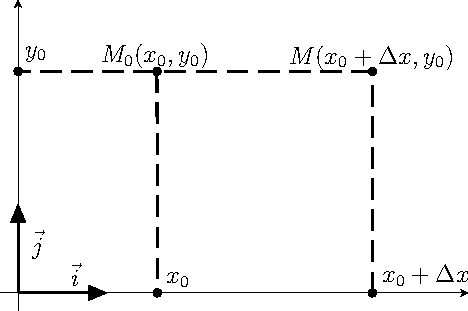
\includegraphics[width=\linewidth]{2.pdf}
			\subcaption{ }
			\label{fig:2.11.1.1}
		\end{minipage}
		\begin{minipage}{0.32\linewidth}
			\centering
			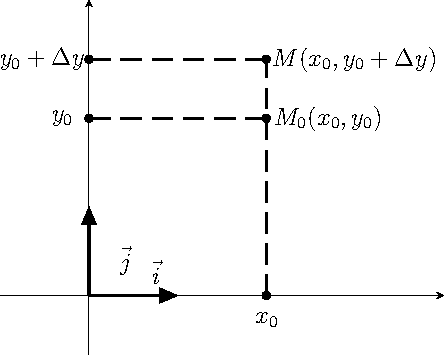
\includegraphics[width=\linewidth]{3.pdf}
			\subcaption{ }
			\label{fig:2.11.1.2}
		\end{minipage}
		\begin{minipage}{0.32\linewidth}
			\centering
			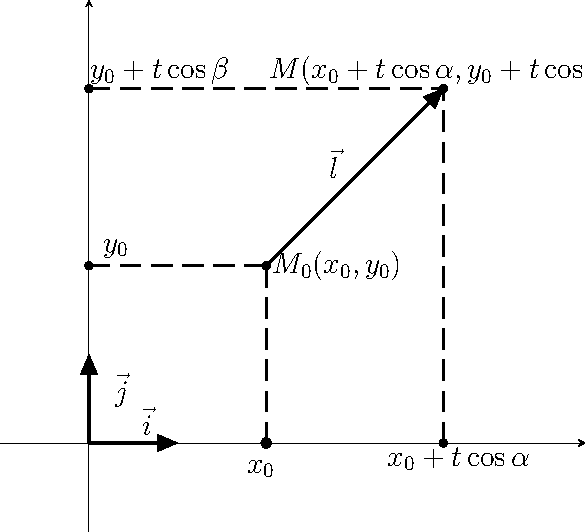
\includegraphics[width=\linewidth]{4.pdf}
			\subcaption{ }
			\label{fig:2.11.1.3}
		\end{minipage}
		\caption{ }
		\label{fig:2.11.1}
	\end{figure}
\end{tbox}

\begin{tbox}{Теорема о связи производной по направлению с градиентом}
	Если функция $y = f(\vec{x})$ дифференцируема в точке $\vec{x}_0 \in E \subset \mathbb{R}^k$, то существуем производная по любому направлению $\vec{l}$, $\vec{l} \in \mathbb{R}^k$, $||\vec{l} = 1||$, и вычисляется это производная по формуле:
	\begin{equation*}
		\frac{\partial f(\vec{x}_0)}{\partial l} = (\grad f(\vec{x}_0), \, l)
	\end{equation*}
	\subsubsection*{Доказательство}

	Так как функция $y = f(\vec{x})$ дифференцируема в точке $\vec{x}_0$, то ее приращения в этой точке можно представить в виде:
	\begin{equation} \label{eq:6.1}
		\Delta f(\vec{x}_0) = f(\vec{x}) - f(\vec{x}_0) = \left(\vec{A}, \, \Delta \vec{x}\right) + \left(\vec{\alpha}(\Delta \vec{x}), \, \Delta \vec{x}\right),
	\end{equation}
	где $\vec{A} = \grad f(\vec{x}_0)$ -- постоянный вектор, координатами этого вектора является частные производные.
	\begin{equation*}
		\begin{aligned}
			\vec{A} = \left(\frac{\partial f(\vec{x}_0)}{\partial x_1}, \, \frac{\partial f(\vec{x}_0)}{\partial x_2}, ..., \frac{\partial f(\vec{x}_0)}{\partial x_k}\right) && \vec{\alpha}(\Delta \vec{x}) \to \vec{\theta} && \Delta \vec{x} \to \vec{\theta}
		\end{aligned}
	\end{equation*}
	Точку представим в виде:
	\begin{align*}
		\vec{x} = \Delta \vec{x} + \vec{x}_0 = \left[\Delta \vec{x} = t \cdot \vec{l}\,\right] = \vec{x}_0 + t \cdot \vec{l} && \Delta \vec{x} \to \vec{0} \text{, при }t \to 0
	\end{align*}

	Подставим в выражение \cref{eq:6.1}:
	\begin{multline*}
		f(\vec{x}_0 + t \cdot \vec{l}) - f(\vec{x}_0) = \left(\grad f(\vec{x}_0), \, t \cdot \vec{l}\,\right) + \left(\vec{\alpha}(t \cdot \vec{l}), \, t \cdot \vec{l}\,\right) = \\= \left(\grad f(\vec{x}_0), \, \vec{l} \,\right) \cdot t + \left(\vec{\alpha}(t \cdot \vec{l}), \, \vec{l}\,\right) \cdot t
	\end{multline*}
	\[\lim_{t \to 0} \frac{f(\vec{x}_0 + t \cdot \vec{l}) - f(\vec{x}_0)}{t} = \lim_{t \to 0} \left[\left(\grad f(\vec{x}_0), \vec{l}\,\right) + \left(\vec{\alpha}(t \cdot \vec{l}), \vec{l}\,\right)\right] = \left(\grad d \, f(\vec{x}_0), \vec{l}\,\right)\]
\end{tbox}

\subsubsection*{Пример}
Дана функция:
\[ u = xy - z^2 \]

Требуется найти производную этой функции в направлении биссектрисы первого координатного угла \( xoy \) в точке \( M_0(-9, 12, 10) \).

\vspace{0.5em}
\begin{enumerate}
	\item \textbf{Вычисление градиента функции \( u \):}
	\[
	\grad u = \left( \frac{\partial u}{\partial x}, \frac{\partial u}{\partial y}, \frac{\partial u}{\partial z} \right) = y \cdot \vec{i} + x \cdot \vec{j} - 2z \cdot \vec{k}
	\]
	В точке \( M_0 \):
	\[
	\grad u(M_0) = 12 \vec{i} - 9 \vec{j} - 20 \vec{k}
	\]
	\item \textbf{Направление биссектрисы \( xoy \):}\\
	Биссектриса первого координатного угла имеет направляющие косинусы:
	\[
	\cos \alpha = \frac{1}{\sqrt{2}}, \quad \cos \beta = \frac{1}{\sqrt{2}}, \quad \cos \gamma = 0
	\]
	Таким образом, вектор направления:
	\[
	\vec{l} = \left(\cos \alpha, \cos \beta, \cos \gamma\right) = \frac{1}{\sqrt{2}} \vec{i} + \frac{1}{\sqrt{2}} \vec{j}
	\]
	\item \textbf{Производная в направлении \( \vec{l} \):}
	\[
	\frac{\partial u(M_0)}{\partial l} = \left( \grad u(M_0), \vec{l} \,\right) = 12 \cdot \frac{1}{\sqrt{2}} + (-9) \cdot \frac{1}{\sqrt{2}} = \frac{3}{\sqrt{2}}
	\]

	\textbf{Итоговый ответ:}
	\[
	\frac{\partial u(M_0)}{\partial l} = \frac{3}{\sqrt{2}}
	\]
\end{enumerate}
%\begin{figure}[H]
%	\centering
%	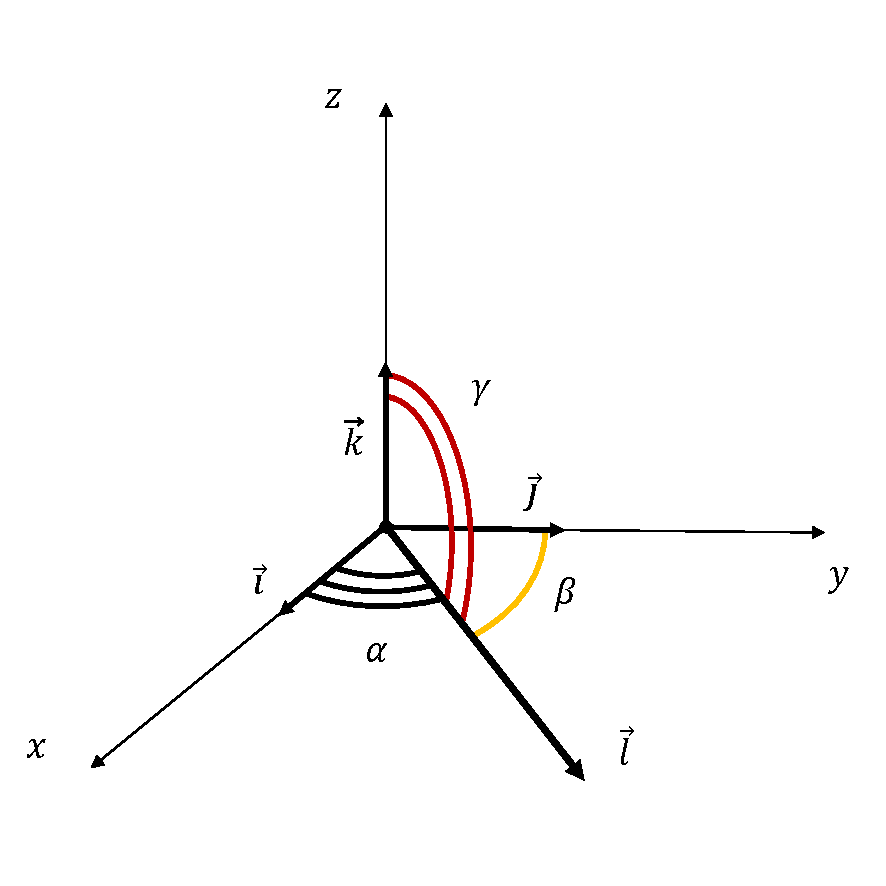
\includegraphics[width=0.5\linewidth]{5.pdf} % Укажите высоту, если нужно
%	\caption{ }
%	\label{fig:18}
%\end{figure}
	\subsection{Условия монотонности функции в заданном направлении.}

\textbf{Определения: } Функция $y = f(\vec{x})$, $\vec{x} \in E \subset \mathbb{R}^k$, называется монотонно возрастающей в точке $\vec{x}_0 \in E \subset \mathbb{R}^k$ в направлении вектора $\vec{l} \subset \mathbb{R}^k$, $||\vec{l}|| = 1$, если существует окрестность точки $x_0$, такая, что для любых точке $\vec{x}_1$ и $\vec{x}_2$, $\forall \vec{x}_1$ и $\forall \vec{x}_2$ из этой окрестности, лежащиз на отрезке коллинеарным с вектором $\vec{l}$, так что $\vec{x}_1$ предшествует $\vec{x}_0$, а $\vec{x}_2$ следует за $\vec{x}_0$, выполняется неравенство.
\begin{equation} \label{eq:6.2}
	f(\vec{x}_1) < f(\vec{x}_0) \quad \text{ и } \quad f(\vec{x}_0) < f(\vec{x}_2)
\end{equation}

Если знак неравенства поменять на противоположный, то:
\begin{equation} \label{eq:6.3}
	f(\vec{x}_1) > f(\vec{x}_0) \quad \text{ и } \quad f(\vec{x}_0) > f(\vec{x}_2)
\end{equation}
получим определение функции монотонно убывающей в точке $\vec{x}_0$ в направлении $\vec{l}$.

\begin{tbox}{Теорема (Без доказательства)}
	Достаточное условие монотонности функции в заданном направлении.

	Пусть $y = f(\vec{x})$, дифференцируема в точке $\vec{x}_0 \in E \subset \mathbb{R}^k$,  $||\vec{l}|| = 1$, $\vec{l} \subset \mathbb{R}^k$ задает направление.

	\begin{itemize}
		\item Если $\displaystyle \frac{\partial \, F(\vec{x}_0)}{\partial l} > 0$, то функция $f(\vec{x})$ является монотонно возрастающей в точке $\vec{x}_0$ в направлении вектора $\vec{l}$.
		\item Если $\displaystyle\frac{\partial f(\vec{x}_0)}{\partial l} < 0$, то функция $f(\vec{x})$ является монотонно убывающей в точке $\vec{x}_0$ в направлении вектора $\vec{l}$.
		\item Если $\displaystyle\frac{\partial f(\vec{x}_0)}{\partial l} = 0$, то функция $f(\vec{x})$ не изменяется в направлении вектора $\vec{l}$, то есть равна $const$.
	\end{itemize}
\end{tbox}
	\subsection{Геометрический смысл градиента}
Пусть $y = f(\vec{x})$, производная по направлению $\vec{l}$ ($\vec{l} \in \mathbb{R}^k$, $||\vec{l}|| = 1$) в точке $\vec{x}_0$ вычисляется по формуле:
\begin{align*}
	\frac{\partial f(\vec{x}_0)}{\partial l} = \left(\grad \, f(\vec{x}_0), \, \vec{l}\right) = ||\grad \, f(\vec{x}_0)|| \cdot ||\vec{l}|| \cdot \cos \omega && \omega = \widehat{\left(\grad \, f(\vec{x}_0), \vec{l}\right)}
\end{align*}
\begin{equation*}
	\boxed{\frac{\partial f(\vec{x}_0)}{\partial l} = ||\grad \, f(\vec{x}_0)|| \cdot \cos \omega}
\end{equation*}

\begin{enumerate}
	\item Пусть $\grad \, f(\vec{x}_0) \uparrow \uparrow \vec{l}$, то $\omega = 0$, $\cos \omega = 1$.
	\begin{equation*}
		\frac{\partial \, f(\vec{x}_0)}{\partial l} = ||\grad \, f(\vec{x}_0)|| > 0.
	\end{equation*}

	В направлении вектора $\grad \, f(\vec{x}_0)$ -- функция монотонно возрастает, при этом производная по направлению принимает \textbf{максимальное} значение, это означает, что в направлении вектора $\grad \, f(\vec{x}_0)$ -- функция быстрее всего возрастает из точки $x_0$, поэтому вектор $\grad \, f(\vec{x}_0)$ определяет наибыстрейший подъема функции из точки $x_0$.

	\item Пусть $\grad \, f(\vec{x}_0) \uparrow \downarrow \vec{l}$, то $\omega = \pi$, $\cos \omega = -1$.
	\begin{equation*}
		\frac{\partial \, f(\vec{x}_0)}{\partial l} = -||\grad \, f(\vec{x}_0)|| < 0.
	\end{equation*}

	Тогда по теореме в направлении противоположному вектору $\grad \, f(\vec{x}_0)$ функция будет монотонно убывать, причем в направлении наибыстрейшего спуска функции из точки $x_0$, так как:
	\begin{equation*}
		\left|\frac{\partial f(\vec{x}_0)}{\partial l}\right| = \left|\grad \, f(\vec{x}_0)\right|
	\end{equation*}
	-- принимает модуль максимальное значение.
	\item Пусть $\grad \, f(\vec{x}_0) \perp \vec{l}$, то $\omega = \frac{\pi}{2}$, $\cos \omega = 0$.
	\begin{equation*}
		\frac{\partial \, f(\vec{x}_0)}{\partial l} = 0.
	\end{equation*}
	То есть по направлению перпендикулярном градиенту $\grad \, f(\vec{x}_0)$, получается что функция $f(\vec{x})$ в точке $\vec{x}_0$ функция не изменяется.
\end{enumerate}

	\subsection{Экстремум функции многих переменных}

\begin{tbox}{Определение 1}
	Функция $y = f(\vec{x})$ имеет в точке $\vec{x}_0 \subset \mathbb{R}^k$ локальный максимум, если существует окрестность точки $\vec{x}_0$, такая, что для $\forall \vec{x}$ из этой окрестности выполняется неравенство:
	\begin{equation*}
		f(\vec{x}) < f(\vec{x}_0)
	\end{equation*}
	\begin{equation}\label{eq:6.4}
		(\exists \delta > 0)(\forall \vec{x} \in E, \, 0 < ||\vec{x} - \vec{x}_0|| < \delta): \, f(\vec{x}) < f(\vec{x}_0)
	\end{equation}
\end{tbox}

Если в определении 1 неравенство нестрогое: $f(\vec{x}) <= f(\vec{x}_0)$ -- то максимум называется \textbf{нестрогим}, аналогично $f(\vec{x})$ -- имеет в точке $\vec{x}_0$ -- локальный минимум, если:
\begin{equation} \label{eq:6.5}
	(\exists \delta > 0)(\forall \vec{x} \in E, \, 0 < ||\vec{x} - \vec{x}_0|| < \delta): \, f(\vec{x}) > f(\vec{x}_0)
\end{equation}

Если неравенство \cref{eq:6.5} нестрогое $f(\vec{x}) >= f(\vec{x}_0)$ -- то минимум называется нестрогим.

\begin{tbox}{Теорема 1. Необходимое условие экстремума}
	Пусть функция \( y = f(x) \) дифференцируема в точке \( \vec{x}_0 \in \mathbb{E} \subset \mathbb{R}^k \) и имеет в этой точке локальный экстремум (максимум или минимум).

	Тогда все частные производные 1-го порядка равны нулю в этой точке:
	\begin{equation*}
		\frac{\partial f(x_0)}{\partial x_1} = 0, \quad \frac{\partial f(x_0)}{\partial x_2} = 0, \quad \dots \quad \frac{\partial f(x_0)}{\partial x_k} = 0.
	\end{equation*}

	\textbf{Доказательство: } Пусть $\vec{x}_0 = (x_{0_1}, x_{0_2}, \cdots, x_{0_k})$,
\end{tbox}

Рассмотрим функцию \( y = f(x_1, x_2, \dots, x_k) \). Зафиксируем переменные \( x_2, x_3, \dots, x_k \), полагая их равными:
\begin{equation}
	x_2 = x_0, \quad x_3 = x_0, \quad \dots, \quad x_k = x_0.
\end{equation}

Тогда получаем функцию \( g \), которая зависит от одной переменной \( x_1 \):
\begin{equation}
	y = f(x_1, x_0, \dots, x_0) = g(x_1).
\end{equation}

\begin{tbox}{Необходимое условие для функции одной переменной}
	Так как точка \( x_0 \) является точкой экстремума для функции \( y = f(x_1, x_2, \dots, x_k) \), то она также является точкой экстремума для функции \( g(x_1) \). Согласно необходимому условию экстремума:
	\begin{equation}
		\frac{dg(x_0)}{dx_1} = 0 \Rightarrow \frac{\partial f(x_0)}{\partial x_1} = 0.
	\end{equation}
\end{tbox}

Аналогично, фиксируя другие переменные, получаем:
\begin{equation}
	\frac{dg(x_0)}{dx_2} = 0 \Rightarrow \frac{\partial f(x_0)}{\partial x_2} = 0.
\end{equation}

Таким образом, все частные производные 1-го порядка равны нулю в точке экстремума.

	\subsection{Понятие квадратичной формы и критерии Сильвестра}

\begin{tbox}{Квадратичная форма}
	Рассмотрим симметрическую матрицу размером $k \times k$:
	\begin{equation*}
		A =
		\begin{pmatrix}
			a_{11} & a_{12} & a_{13} & \cdots & a_{1k} \\
			a_{21} & a_{22} & a_{23} & \cdots & a_{2k} \\
			a_{31} & a_{32} & a_{33} & \cdots & a_{3k} \\
			\vdots & \vdots & \vdots & \ddots & \vdots \\
			a_{k1} & a_{k2} & a_{k3} & \dots & a_{kk} \\
		\end{pmatrix}
		\quad a_{ij} = a_{ji}
	\end{equation*}

	Главными минорами матрицы $A$ называются следующие определители:
	\begin{align*}
		A_1 = a_{11} &&
		A_2 = \begin{vmatrix}
			a_{11} & a_{12} \\
			a_{21} & a_{22}
		\end{vmatrix} &&
		A_{3} = \begin{vmatrix}
			a_{11} & a_{12} & a_{13} \\
			a_{21} & a_{22} & a_{23} \\
			a_{31} & a_{32} & a_{33}
		\end{vmatrix} &&
		A_k = \begin{vmatrix}
			a_{11} & a_{12} & a_{13} & \cdots & a_{1k} \\
			a_{21} & a_{22} & a_{23} & \cdots & a_{2k} \\
			a_{31} & a_{32} & a_{33} & \cdots & a_{3k} \\
			\vdots & \vdots & \vdots & \ddots & \vdots \\
			a_{k1} & a_{k2} & a_{k3} & \dots  & a_{kk}
		\end{vmatrix}
	\end{align*}

	Пусть $x_1$, $x_2$, $x_3$, $\dots$, $x_k$ -- некоторые переменные величины, из них и элементов матрицы $A$ составим выражения:
	\begin{align*}
		P(x_1, x_2, \dots, x_k) = \,
		& a_{11} \cdot x_{1}^2 + a_{12} \cdot x_{1} x_{2} + a_{13} \cdot x_{1} x_{3} + ... + a_{1k} \cdot x_{1} x_{k} + \\
		&a_{21} \cdot x_{2} x_{1} + a_{22} \cdot x_{2}^2 + a_{23} \cdot x_{2} x_{3} + ... + a_{2k} \cdot x_{2} x_{k} + \\
		&a_{31} \cdot x_{3} x_{1} + a_{32} \cdot x_{3} x_{2} + a_{33} \cdot x_{3}^2 + ... + a_{3k} \cdot x_{3} x_{k} + \\
		&\dots\\
		&a_{k1} \cdot x_{k} x_{1} + a_{k2} \cdot x_{k} x_{2} + a_{k3} \cdot x_{k} x_{3} + ... + a_{kk} \cdot x_{k}^2
	\end{align*}

	Так как матрица $A$ симметрична ($a_{ij} = a_{ji}$), тогда:
	\begin{equation} \label{eq:7.1}
		\begin{aligned}
			P(x_1, x_2, \dots, x_k) = &(a_{11} \cdot x_{1}^2 + a_{22} \cdot x_{2}^2 + a_{33} \cdot x_{3}^2 + ... + a_{kk} \cdot x_k^2) + \\
			&(2 a_{12} \cdot x_1 x_2 + 2 a_{13} \cdot x_1 x_3 + 2 a_{23} \cdot x_2 x_3 + ... + 2 a_{k - 1, k} \cdot x_{k-1} x_{k})
		\end{aligned}
	\end{equation}

	Выражение, включающее в себя квадраты всех переменных и всевозможные их попарные произведения, называется \textbf{квадратичной формой}.
	\begin{align*}
		\text{Пусть $k = 2$} && P(x_1, x_2) = a_{11} \cdot x_1^2 + a_{22} \cdot x_2^2 + 2 a_{12} \cdot x_1 x_2,\\
		\text{Пусть $k = 3$} && P(x_1, x_2, x_3) = a_{11} \cdot x_1^2 + a_{22} \cdot x_2^2 + a_{33} \cdot x_3^2 + \\&&+ 2 a_{12} \cdot x_1 x_2 + 2 a_{13} \cdot x_1 x_3 + 2 a_{23} \cdot x_2 x_3
	\end{align*}

	Если квадратичная форма \eqref{eq:7.1}, $P(x_1, x_2, ..., x_k) > 0$, при различных значения переменных, то ее называют \textbf{положительно определенной квадратичной формой}.

	Если $P(x_1, x_2, ..., x_k) < 0$, при всех значениях переменных $(x_1, x_2, ..., x_k)$, то ее называют \textbf{отрицательно определенной квадратичной формой}.

	Если $P(x_1, x_2, ..., x_k)$ принимает как положительное, так и отрицательное значение, при разных значениях переменных, то ее называют \textbf{знакопеременной квадратичной формой}.
\end{tbox}

\begin{tbox}{Критерии Сильвестра}
	Чтобы квадратичная форма матрицы $A$, являлась \textit{положительной определенной}, необходимо и достаточно, чтобы все главные миноры матрицы $A$ были положительны.

	\begin{equation*}
		P(x_1, x_2, ... x_k) > 0  \Leftrightarrow A_1 > 0, \, A_2 > 0, \, A_3 > 0, \, ...,A_k>0
	\end{equation*}

	Чтобы квадратичная форма матрицы $A$, являлась \textit{отрицательно определенной}, необходимо и достаточно, чтобы все знаки главных миноров матрицы $A$ чередовались, при чем $A_1 < 0$.

	\begin{equation*}
		P(x_1, x_2, ..., x_k) < 0 \Leftrightarrow A_1 < 0, \, A_2 > 0, \, A_3 < 0, ..., \, A_k > 0
	\end{equation*}
\end{tbox}

\begin{tbox}{Второй дифференциал функции многих переменных}
	Рассмотрим второй дифференциал для функции $k$ - независимых переменных.
	\begin{multline*}
		d^2 y = \left(\frac{\partial}{\partial x_1} dx_1 + \frac{\partial}{\partial x_2} dx_2 + \cdots + \frac{\partial}{\partial x_k} dx_k\right)^2 f(x_1, \ldots, x_k) \\
		= \left(\frac{\partial^2}{\partial x_1^2} dx_1^2 + \frac{\partial^2}{\partial x_2^2} dx_2^2 + \cdots + \frac{\partial^2}{\partial x_k^2} dx_k^2 \right. \\
		\left. + 2\frac{\partial^2}{\partial x_1 \partial x_2} dx_1 dx_2 + \cdots + 2\frac{\partial^2}{\partial x_{k-1} \partial x_k} dx_{k-1} dx_k\right) f \\
		= \frac{\partial^2 f}{\partial x_1^2} dx_1^2 + \frac{\partial^2 f}{\partial x_2^2} dx_2^2 + \cdots + \frac{\partial^2 f}{\partial x_k^2} dx_k^2 \\
		+ 2\frac{\partial^2 f}{\partial x_1 \partial x_2} dx_1 dx_2 + \cdots + 2\frac{\partial^2 f}{\partial x_{k-1} \partial x_k} dx_{k-1} dx_k
	\end{multline*}
	Если $x_0$ - стационарная точка.
	\begin{multline*}
		d^2 y\left(\vec{x}_0\right)= \,\frac{\partial^2 f\left(\vec{x}_0\right)}{\partial x_1^2} d x_1^2+\frac{\partial^2 f\left(\vec{x}_0\right)}{\partial x_2^2} \cdot d x_2^2+...+ \frac{\partial^2 f\left(\vec{x}_0\right)}{\partial x_k^2} \cdot d x_k^2+ \\
		+2\frac{\partial^2 f}{\partial x_1 \partial x_2} d x_1 d x_2+2\frac{\partial^2 f}{\partial x_1 \partial x_3} d x_1 d x_3+\ldots+2\frac{\partial^2 f\left(\vec{x}_0\right)}{\partial x_{k-1} \partial x_k} d x_{k-1} d x_k
	\end{multline*}

	$d^2 y$ в точке $x_0$ -- является квадратичной формой относительно дифференциалов независимых переменных $d x_1$, $d x_2$, ..., $d x_k$. Матрица этой квадратичной формы имеет вид:
	\begin{equation*}
		\begin{aligned}
			A = \begin{pmatrix}
				\frac{\partial^2 f}{\partial x_1^2} & \frac{\partial^2 f}{\partial x_1 \partial x_2} & \frac{\partial^2 f}{\partial x_1 \partial x_3} & \cdots & \frac{\partial^2 f}{\partial x_1 \partial x_k} \\
				\frac{\partial^2 f}{\partial x_2 \partial x_1} & \frac{\partial^2 f}{\partial x_2^2} & \frac{\partial^2 f}{\partial x_2 \partial x_3} & \cdots & \frac{\partial^2 f}{\partial x_2 \partial x_k} \\
				\vdots & \vdots & \vdots & \ddots & \vdots \\
				\frac{\partial^2 f}{\partial x_k \partial x_1} & \frac{\partial^2 f}{\partial x_k \partial x_2} & \frac{\partial^2 f}{\partial x_k \partial x_3} & \cdots & \frac{\partial^2 f}{\partial x_k \partial x_k} \\
			\end{pmatrix}
		\end{aligned}
	\end{equation*}

	Тогда для определения знака $d^2 y (\vec{x}_0)$ -- применяем критерий Сильвестра. Для этого находим в точке $\vec{x}_0$ -- главные миноры матрицы $A$ и определяет их знак, соответственно делаем вывод о знаке квадратичной формы.
\end{tbox}

\begin{tbox}{Теорема о достаточном условии вывода экстремума для функции двух переменных}
	Пусть функция $z = f(x,y)$ -- дифференцируемая в окрестностях стационарной точки $M_0(x_0, y_0)$ и имеет в этой точке непрерывную частную производную второго порядка. Тогда:
	\begin{enumerate}
		\item Если $f_{xx}''(M_0) \cdot f_{yy}''(M_0) - {f_{xy}''}^2(M_0) >0$ и $f_{xx}''(M_0) > 0$, то $M_0$ -- точка минимума.
		\item Если $f_{xx}''(M_0) \cdot f_{yy}''(M_0) - {f_{xy}''}^2(M_0) >0$ и $f_{xx}''(M_0) < 0$, то $M_0$ -- точка максимума.
		\item Если $f_{xx}''(M_0) \cdot f_{yy}''(M_0) - {f_{xy}''}^2(M_0) < 0$, то в точке $M_0$ экстремума нет.
	\end{enumerate}

	\subsubsection*{Доказательство}
	Следует из критерия Сильвестра, для этого запишем второй дифференциал функции $z = f(x,y)$ в стационарной точке $M_0$.
	\begin{equation*}
		\begin{aligned}
			d^2 z (M_0) = f_{xx}''(M_0) \,dx^2 + 2 f_{xy}''(M_0) \,dx\, dy + f_{yy}''(M_0) \, dy^2
		\end{aligned}
	\end{equation*}
	$d^2 z(M_0)$ -- является квадратичной формой относительно дифференциалов $dx$ и $dy$, а матрица этой квадратичной формы имеет вид.
	\begin{equation*}
		\begin{aligned}
			A = \begin{pmatrix}
				f_{xx}''(M_0) & f_{xy}''(M_0) \\
				f_{yx}''(M_0) & f_{yy}''(M_0)
			\end{pmatrix}
		\end{aligned}
	\end{equation*}

	Запишем главные миноры матрицы $A$:
	\begin{equation*}
		\begin{aligned}
			A_1 = f_{xx}''(M_0) && A_2 = \begin{vmatrix}
				f_{xx}''(M_0) & f_{xy}''(M_0) \\
				f_{yx}''(M_0) & f_{yy}''(M_0)
			\end{vmatrix} = f_{xx}''(M_0) \cdot f_{yy}''(M_0) - {f_{xy}''}^2(M_0)
		\end{aligned}
	\end{equation*}

	Тогда по критерию Сильвестра:
	\begin{enumerate}
		\item если $A_1 > 0$ и $A_2 > 0$, то квадратичная форма является \textit{положительно определенной}, т.е. $d^2 z(M_0) > 0$ и по теореме 2 точка $M_0$ является точкой \textit{минимума}.
		\item если $A_1 < 0$ и $A_2 > 0$, то квадратичная форма является \textit{отрицательно определенной}, т.е. $d^2 z(M_0) < 0$ и по теореме 2 точка $M_0$ является точкой \textit{максимума}.
		\item если $A_2 = f_{xx}''(M_0) \cdot f_{yy}''(M_0) - {f_{xy}''}^2(M_0) < 0$, в этом случае квадратичная форма является знакопеременной квадратичной формой, т.к. оно не будет ни положительной, ни отрицательной.
	\end{enumerate}

	Если $d^2 z (M_0)$ -- не определен по знаку, то поп теореме 3 в точке $M_0$ экстремума нет. \\

	\textbf{Замечания: } В случае, если $A_2 = f_{xx}''(M_0) \cdot f_{yy}''(M_0) - {f_{xy}''}^2(M_0) = 0$, то наличия или отсутствие экстремума необходимо доказать по определению, этот случай соответствует тому, что $d^2 z(M_0) = 0$.
\end{tbox}
	\subsection{Условный экстремум функции многих переменных}
\begin{tbox}{Условный экстремум}
	Экстремум функции, на аргументы которой наложены дополнительные условия связи, называется \textbf{условным экстремумом}.
\end{tbox}

\begin{figure}[h]
	\centering
	\begin{minipage}[c]{0.4\linewidth} % [c] для выравнивания по центру
		\centering
		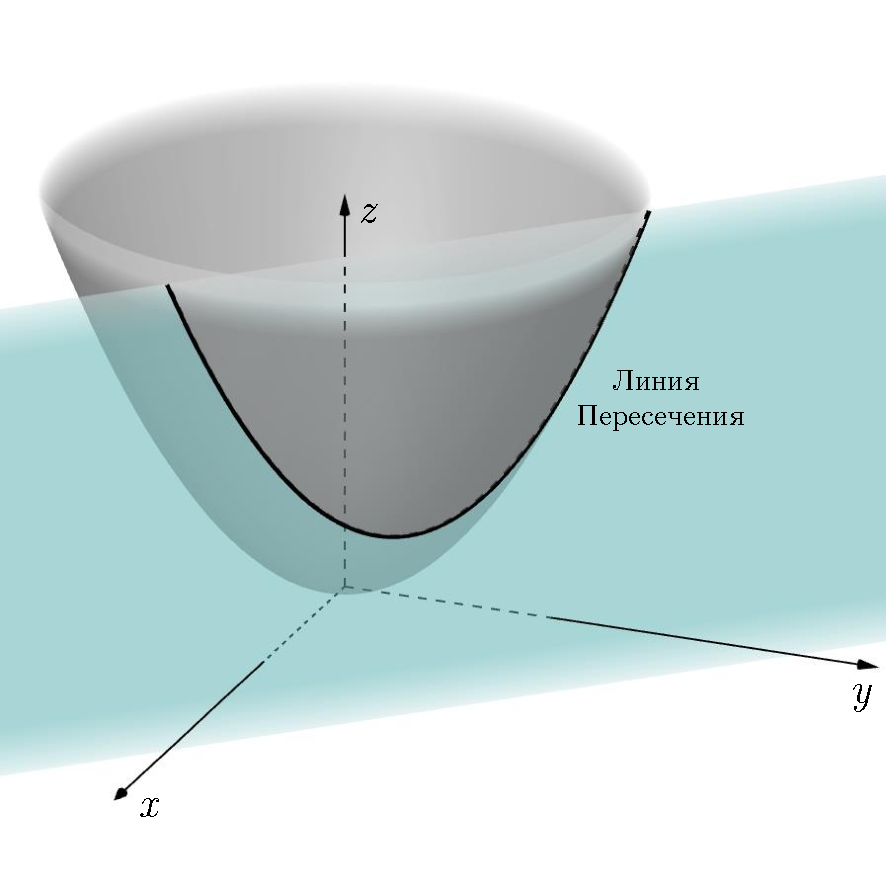
\includegraphics[width=\linewidth]{7.pdf} % Укажите высоту, если нужно
		\caption{Графическая иллюстрация условного экстремума}
		\label{fig:17}
	\end{minipage}
\end{figure}

\subsubsection*{Пример условного экстремума (Рис. \ref{fig:17})}
Пусть $z = x^2 + y^2$ при условии связи $x + y = 1$. Точка $M_0(0, 0)$ является точкой минимума (абсолютный экстремум).

Экстремум на линии пересечения плоскости $x + y = 1$ и параболоида $z = x^2 + y^2$ является условным экстремумом. Для его нахождения выразим переменную $y$ из условия связи и подставим в уравнение функции.

Получаем функцию одной независимой переменной, которую исследуем на экстремум:
\begin{gather*}
	x + y = 1 \Rightarrow y = 1 - x, \\
	z = x^2 + y^2 = x^2 + (1 - x)^2 = x^2 + 1 - 2x + x^2 = 2x^2 - 2x + 1.
\end{gather*}
\begin{align*}
	z_x' &= 4x - 2 = 0 \Rightarrow x = \frac{1}{2} \text{ — стационарная точка}, \\
	z_{xx}'' &= 4 > 0 \Rightarrow x = \frac{1}{2} \text{ — точка минимума функции } z = 2x^2 - 2x + 1, \\
	y &= 1 - x = 1 - \frac{1}{2} = \frac{1}{2}; \quad \left(\frac{1}{2}; \frac{1}{2}\right) \text{ — точка условного минимума}, \\
	z_{\text{min}} &= z\left(\frac{1}{2}; \frac{1}{2}\right) = \left(\frac{1}{2}\right)^2 + \left(\frac{1}{2}\right)^2 = \frac{1}{2}.
\end{align*}

Если уравнений связи несколько или они нелинейные, то свести задачу условного экстремума к исследованию функций одной или нескольких переменных бывает сложно. В этом случае применяют \textit{метод неопределённых множителей Лагранжа}.

\begin{tbox}{Метод множителей Лагранжа}
	В общем случае задача ставится следующим образом:

	Пусть задана функция $y = f(x_1, x_2, \dots, x_k)$, а независимые переменные $x_1, x_2, \dots, x_k$ связаны условиями, число которых меньше числа независимых переменных:
	\begin{equation} \label{eq:8.1}
		\begin{cases}
			\varphi_1(x_1, x_2, \dots, x_k) = 0, \\
			\varphi_2(x_1, x_2, \dots, x_k) = 0, \\
			\dots, \\
			\varphi_n(x_1, x_2, \dots, x_k) = 0,
		\end{cases}
		\quad n < k.
	\end{equation}

	Составим функцию Лагранжа:
	\begin{multline} \label{eq:8.2}
		L = f(x_1, x_2, \dots, x_k) + \lambda_1 \varphi_1(x_1, x_2, \dots, x_k) + \lambda_2 \varphi_2(x_1, x_2, \dots, x_k) + \dots \\ \dots + \lambda_n \varphi_n(x_1, x_2, \dots, x_k).
	\end{multline}

	Здесь $\lambda_1, \lambda_2, \dots, \lambda_n$ — неопределённые множители Лагранжа, которые находятся из условий:
	\begin{equation*}
		\begin{cases}
			\frac{\partial L}{\partial \lambda_1} = \varphi_1(x_1, x_2, \dots, x_k) = 0, \\
			\frac{\partial L}{\partial \lambda_2} = \varphi_2(x_1, x_2, \dots, x_k) = 0, \\
			\dots, \\
			\frac{\partial L}{\partial \lambda_n} = \varphi_n(x_1, x_2, \dots, x_k) = 0.
		\end{cases}
	\end{equation*}

	Задача поиска условного экстремума сводится к поиску обычного экстремума для функции Лагранжа \eqref{eq:8.2}. Необходимое условие экстремума:
	\begin{equation} \label{eq:8.3}
		\begin{cases}
			\frac{\partial L}{\partial x_1} = 0, \\
			\frac{\partial L}{\partial x_2} = 0, \\
			\dots, \\
			\frac{\partial L}{\partial x_k} = 0, \\
			\frac{\partial L}{\partial \lambda_1} = \varphi_1(x_1, x_2, \dots, x_k) = 0, \\
			\frac{\partial L}{\partial \lambda_2} = \varphi_2(x_1, x_2, \dots, x_k) = 0, \\
			\dots, \\
			\frac{\partial L}{\partial \lambda_n} = \varphi_n(x_1, x_2, \dots, x_k) = 0.
		\end{cases}
	\end{equation}

	Получаем систему $k + n$ уравнений относительно неизвестных $x_1, x_2, \dots, x_k$ и $\lambda_1, \lambda_2, \dots, \lambda_n$.

	Решая систему \eqref{eq:8.3}, находим стационарные точки $M_0(x_{0_1}, x_{0_2}, \dots, x_{0_k})$ и значения множителей Лагранжа $\lambda_1 = \lambda_{0_1}, \lambda_2 = \lambda_{0_2}, \dots, \lambda_n = \lambda_{0_n}$.
\end{tbox}

\begin{tbox}{Второй дифференциал функции Лагранжа}
	Дальнейшее исследование стационарных точек на экстремум связано с анализом знака второго дифференциала с учётом дифференциальных условий связи.

	Второй дифференциал функции Лагранжа в точке $M_0$:
	\begin{equation*}
		\begin{aligned}
			d^2 L(M_0) = &\frac{\partial^2 L(M_0)}{\partial x_1^2} dx_1^2 + \frac{\partial^2 L(M_0)}{\partial x_2^2} dx_2^2 + \dots + \frac{\partial^2 L(M_0)}{\partial x_k^2} dx_k^2 \, + \\
			&+ 2 \frac{\partial^2 L(M_0)}{\partial x_1 \partial x_2} dx_1 dx_2 + 2 \frac{\partial^2 L(M_0)}{\partial x_1 \partial x_3} dx_1 dx_3 + \dots + 2 \frac{\partial^2 L(M_0)}{\partial x_{k-1} \partial x_k} dx_{k-1} dx_k.
		\end{aligned}
	\end{equation*}

	Так как переменные $x_1, x_2, \dots, x_k$ связаны условиями \eqref{eq:8.1}, их дифференциалы также связаны. Найдём дифференциалы условий связи в точке $M_0$:
	\begin{gather*}
		\varphi_1(x_1, x_2, \dots, x_k) = 0 \quad \Big| \, d, \\
		d\varphi_1(M_0) = \frac{\partial \varphi_1(M_0)}{\partial x_1} dx_1 + \frac{\partial \varphi_1(M_0)}{\partial x_2} dx_2 + \dots + \frac{\partial \varphi_1(M_0)}{\partial x_k} dx_k = \sum_{i=1}^k \frac{\partial \varphi_1(M_0)}{\partial x_i} dx_i = 0, \\
		\varphi_2(x_1, x_2, \dots, x_k) = 0 \quad \Big| \, d, \\
		d\varphi_2(M_0) = \frac{\partial \varphi_2(M_0)}{\partial x_1} dx_1 + \frac{\partial \varphi_2(M_0)}{\partial x_2} dx_2 + \dots + \frac{\partial \varphi_2(M_0)}{\partial x_k} dx_k = \sum_{i=1}^k \frac{\partial \varphi_2(M_0)}{\partial x_i} dx_i = 0, \\
		\dots, \\
		\varphi_n(x_1, x_2, \dots, x_k) = 0 \quad \Big| \, d, \\
		d\varphi_n(M_0) = \frac{\partial \varphi_n(M_0)}{\partial x_1} dx_1 + \frac{\partial \varphi_n(M_0)}{\partial x_2} dx_2 + \dots + \frac{\partial \varphi_n(M_0)}{\partial x_k} dx_k = \sum_{i=1}^k \frac{\partial \varphi_n(M_0)}{\partial x_i} dx_i = 0.
	\end{gather*}

	Исследуем знак второго дифференциала с учётом этих условий.
\end{tbox}

\subsubsection*{Пример метода множителей Лагранжа}
Задана функция $z = x^2 + xy + y^2$ с условием $x + y = 2$, где $x$ и $y$ — независимые переменные. Введём функцию Лагранжа:
\[
L = x^2 + xy + y^2 + \lambda(x + y - 2).
\]

Частные производные:
\[
\begin{cases}
	2x + y + \lambda = 0, \\
	x + 2y + \lambda = 0, \\
	x + y = 2.
\end{cases}
\]

Решаем систему:
\[
y = 2 - x, \quad 2x + (2 - x) + \lambda = 0, \quad x + 2(2 - x) + \lambda = 0.
\]
\[
x = 1, \quad y = 1, \quad \lambda = -3.
\]

Вторые производные:
\[
\frac{\partial^2 L}{\partial x^2} = 2, \quad \frac{\partial^2 L}{\partial x \partial y} = 1, \quad \frac{\partial^2 L}{\partial y^2} = 2.
\]

Квадратичная форма:
\[
d^2 L = 2 dx^2 + 2 dx dy + 2 dy^2.
\]
При $dx + dy = 0$ (так как $x + y = 2$):
\[
d^2 L = 2 dx^2 > 0.
\]

Точка $(1, 1)$ — условный минимум. Значение:
\[
z(1, 1) = 3.
\]

\textbf{Ответ:} $z_{\text{min}} = 3$ в точке $(1, 1)$.
\end{document}